\documentclass[12pt, a4paper]{article}
\usepackage{ctex}
\usepackage{amsmath,amscd,amsbsy,amssymb,latexsym,url,bm,amsthm}
\usepackage{caption}
\usepackage{epsfig,graphicx,subfigure}
\usepackage{enumitem,balance}
\usepackage{wrapfig}
\usepackage{listings}
\usepackage{mathrsfs,euscript}
\usepackage[usenames]{xcolor}
\usepackage{hyperref}
\usepackage[vlined,ruled,linesnumbered]{algorithm2e}
\hypersetup{colorlinks=true,linkcolor=black}

\captionsetup[figure]{
	labelfont = {bf},
	labelformat = {default},
	labelsep = period,
	name = {Fig.}
}

\newtheorem{theorem}{Theorem}
\newtheorem{lemma}[theorem]{Lemma}
\newtheorem{proposition}[theorem]{Proposition}
\newtheorem{corollary}[theorem]{Corollary}
\newtheorem{exercise}{Exercise}
\newtheorem*{solution}{Solution}
\newtheorem{definition}{Definition}
\theoremstyle{definition}
\lstset{
	keywordstyle = \color{blue!70}\bfseries, 
	basicstyle = \ttfamily, 
	commentstyle = \ttfamily,
	showstringspaces = false,
	frame = shadowbox,
	rulesepcolor = \color{red!20!green!20!blue!20},
}

\renewcommand{\thefootnote}{\fnsymbol{footnote}}

\newcommand{\postscript}[2]{
	\setlength{\epsfxsize}{#2\hsize}
  	\centerline{\epsfbox{#1}}
}

\renewcommand{\baselinestretch}{1.0}

\setlength{\oddsidemargin}{-0.35in}
\setlength{\evensidemargin}{-0.35in}
\setlength{\topmargin}{-0.3in}
\setlength{\headheight}{0in}
\setlength{\headsep}{0in}
\setlength{\textheight}{10.2in}
\setlength{\textwidth}{7in}
\makeatletter 
\renewenvironment{proof}[1][Proof] {\par\pushQED{\qed}\normalfont\topsep6\p@\@plus6\p@\relax\trivlist\item[\hskip\labelsep\bfseries#1\@addpunct{.}]\ignorespaces}{\popQED\endtrivlist\@endpefalse} \makeatother
\makeatletter
\renewenvironment{solution}[1][Solution] {\par\pushQED{\qed}\normalfont\topsep6\p@\@plus6\p@\relax\trivlist\item[\hskip\labelsep\bfseries#1\@addpunct{.}]\ignorespaces}{\popQED\endtrivlist\@endpefalse} \makeatother

\begin{document}
\noindent

%========================================================================
\noindent\framebox[\linewidth]{\shortstack[c]{
\Large{\textbf{Lab \#2: QR Code}}\vspace{1mm}\\
EE447 Mobile Network, Luoyi Fu, Spring 2021\\
\textbf{Due}: \textit{Sunday, May 2nd}}}
\begin{center}

Name: Hongjie Fang  \quad Student ID:518030910150 \quad Email: \href{mailto:galaxies@sjtu.edu.cn}{galaxies@sjtu.edu.cn}
\end{center}

\section{Purpose and Objective}\label{section1}
A barcode is an optical machine-readable representation of data relating to the object to which it is attached. Originally barcodes systematically represented data by varying the widths and spacings of parallel lines, which can be viewed as one-dimensional representation. 

Later, two-dimensional representation is developed, and among them, most important and widely used one is QR code, \textit{i.e.}, Quick Response code. QR code has become the most popular encoding methods on mobile devices nowadays, and the QR Code system became popular outside the automotive industry due to its fast readability and greater storage capacity compared to standard UPC barcodes. The applications of QR code include product tracking, item identification, time tracking, document
management, and general marketing.

In this lab, we are given a well-written sample application for QR code encoding and decoding. Basically, what we are required to do is to successfully compile and execute the application in a real-world mobile phone and test for its performance. What's more, I make some critical modifications to make the application handier to users.

\section{Compilation and Execution of the Application}
We use Android Studio to open the project. While automatically configuring the project, the Android Studio found out that the SDK path is not correctly set, as shown in Fig. \ref{fig1}. Click ``OK'', and it will automatically set the correct SDK path for you.

\begin{figure}[htbp]
	\centering
	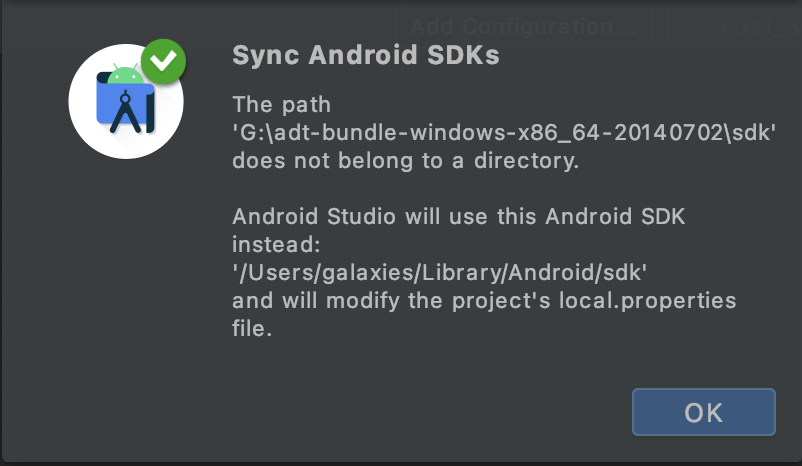
\includegraphics[width=3.5in]{1.png}
	\caption{Android Studio automatically set SDK path}
	\label{fig1}
\end{figure}

Then, from the following lines of the \texttt{build.gradle} for the application, we know that the version of SDK compiler is 21, and the version of the building tools is 23.0.1.
\begin{lstlisting}
    compileSdkVersion 21
    buildToolsVersion "23.0.1"
\end{lstlisting}

Open SDK Manager, and install SDK Platform for Android 5.0 (Lollipop) along with Android SDK build tools of version 23.0.1. Thus, we successfully complete the SDK settings of the project.
\clearpage
Then, we need to fix the gradle version of the project. During this process, many unexpected errors may occur due to different environment of the computer. I compile the application under MacOS Big Sur 11.3, and have encountered the folowing exception as Fig. \ref{fig2} shown.

\begin{figure}[ht]
	\centering
	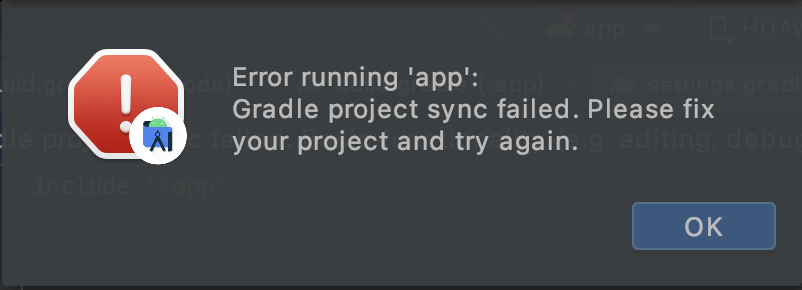
\includegraphics[width=3.5in]{2.png}
	\caption{The exception that I have encountered due to incorrect settings of gradle}
	\label{fig2}
\end{figure}

To solve this, we need first open ``project structure'' and set the Android Gradle Plugin Version to 4.1.3, and set the Gradle Version to 6.5, as Fig. \ref{fig3} shown.
\begin{figure}[htbp]
	\centering
	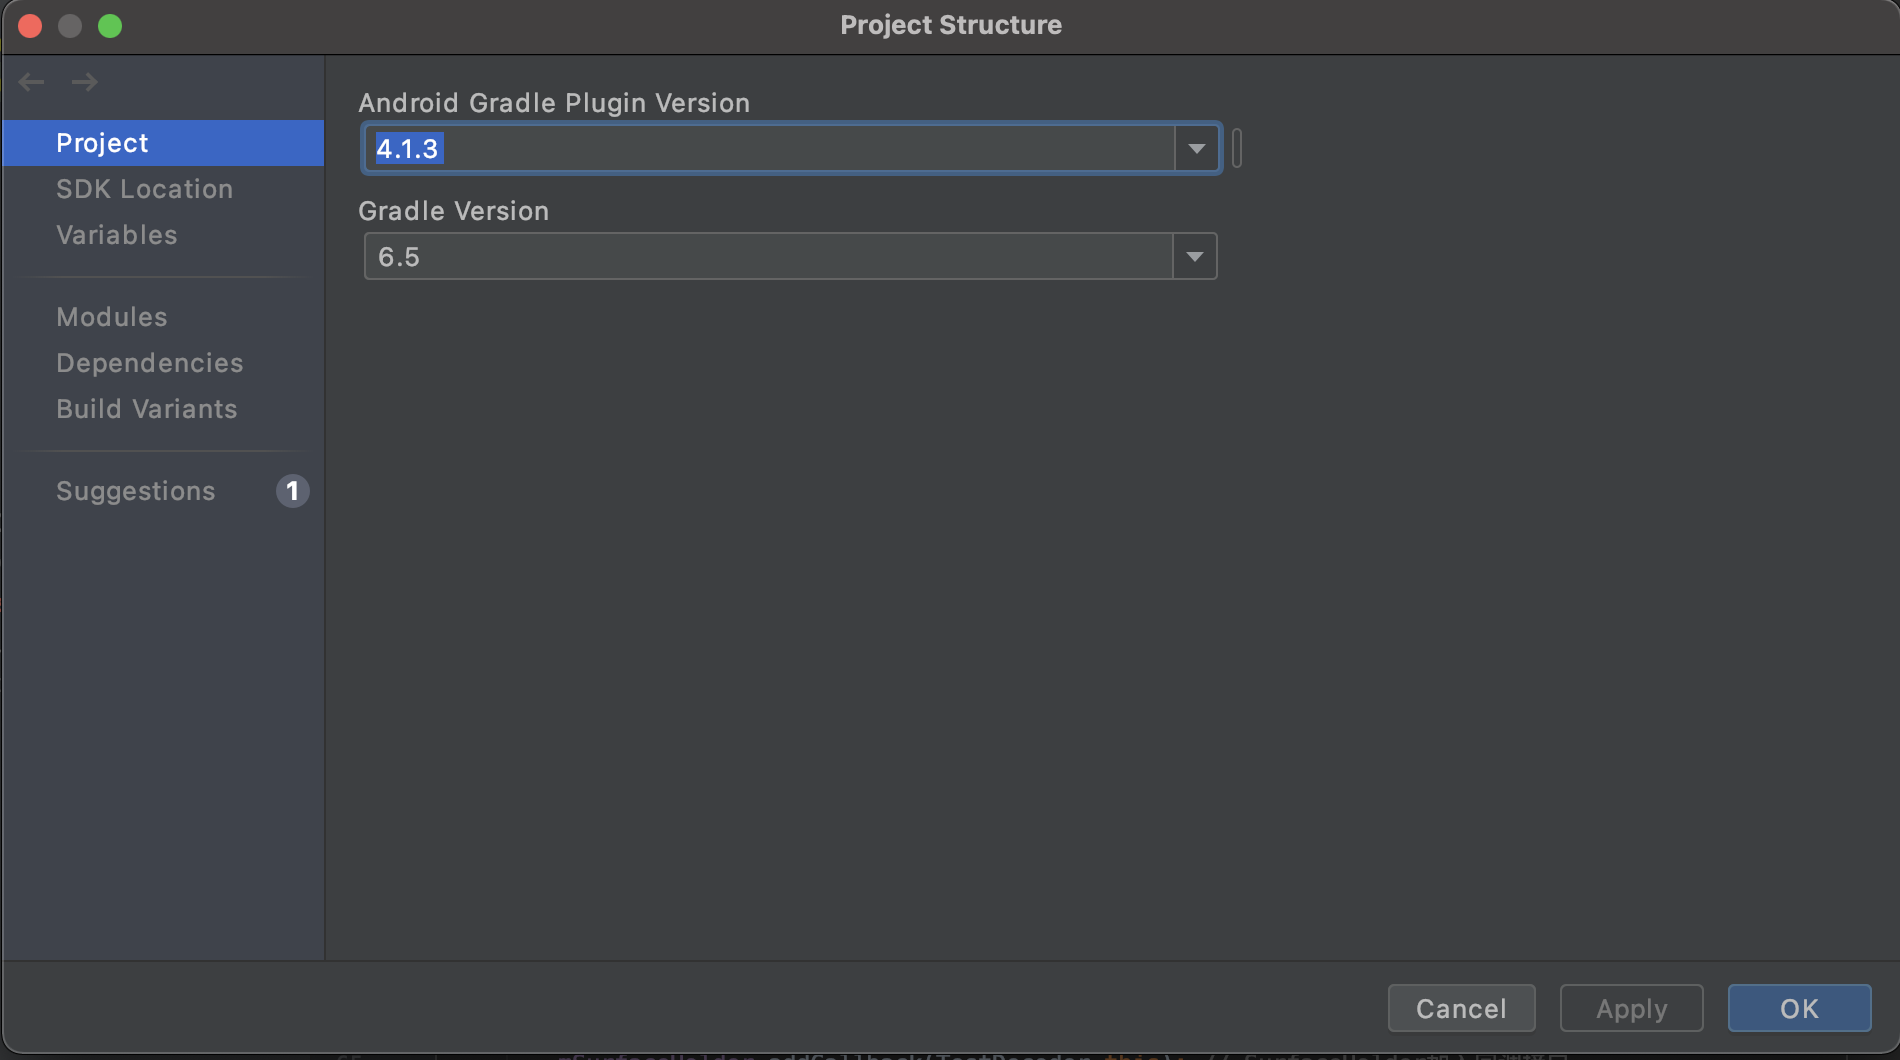
\includegraphics[width=6in]{3.png}
	\caption{The correct gradle configuration}
	\label{fig3}
\end{figure}

Then, the Android Studio will automatically synchronize the project. But unfortunately, we may meet another problem shown as follows.
\begin{figure}[htbp]
	\centering
	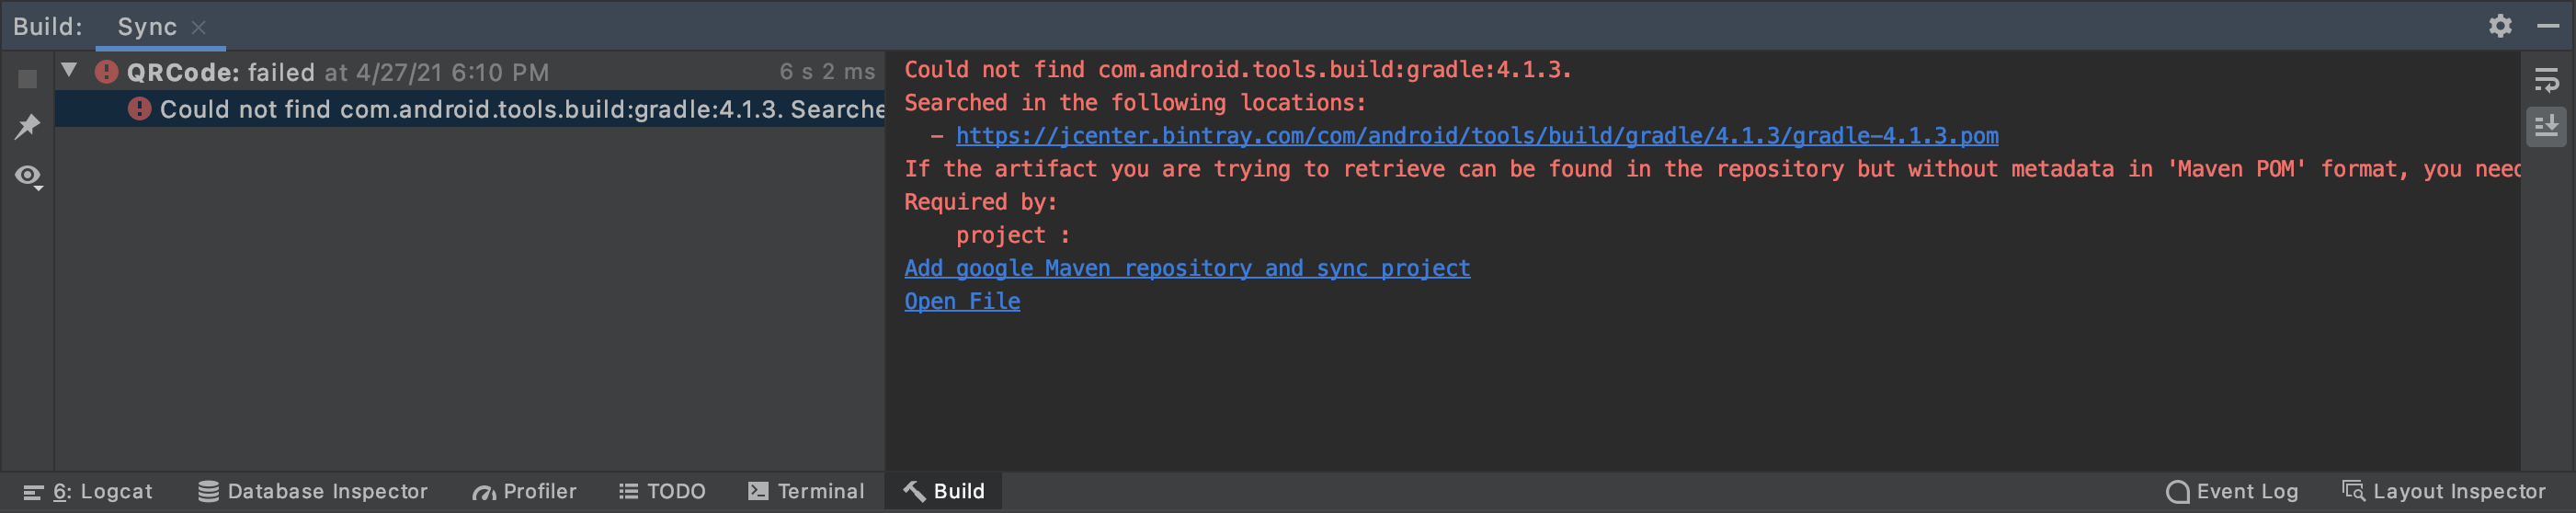
\includegraphics[width=7in]{4.png}
	\caption{The correct gradle configuration}
	\label{fig4}
\end{figure}

The error message indicates that we should add Google Maven repository and synchronize the project again. Therefore, we can click the ``Add google Maven repository and sync project'' and then click ``Do refactor'' to add Maven repository to the project.

After adding Maven repository to the project, the project synchronized successfully. Therefore, we can write the application into a real-world mobile to test the performance.

We use a HUAWEI P20 mobile for real-world testing, and the main function of the initial application is shown in Fig. \ref{fig5}.

\begin{figure}[htbp]
	\centering
		\begin{minipage}[t]{0.25\linewidth}
		\centering
		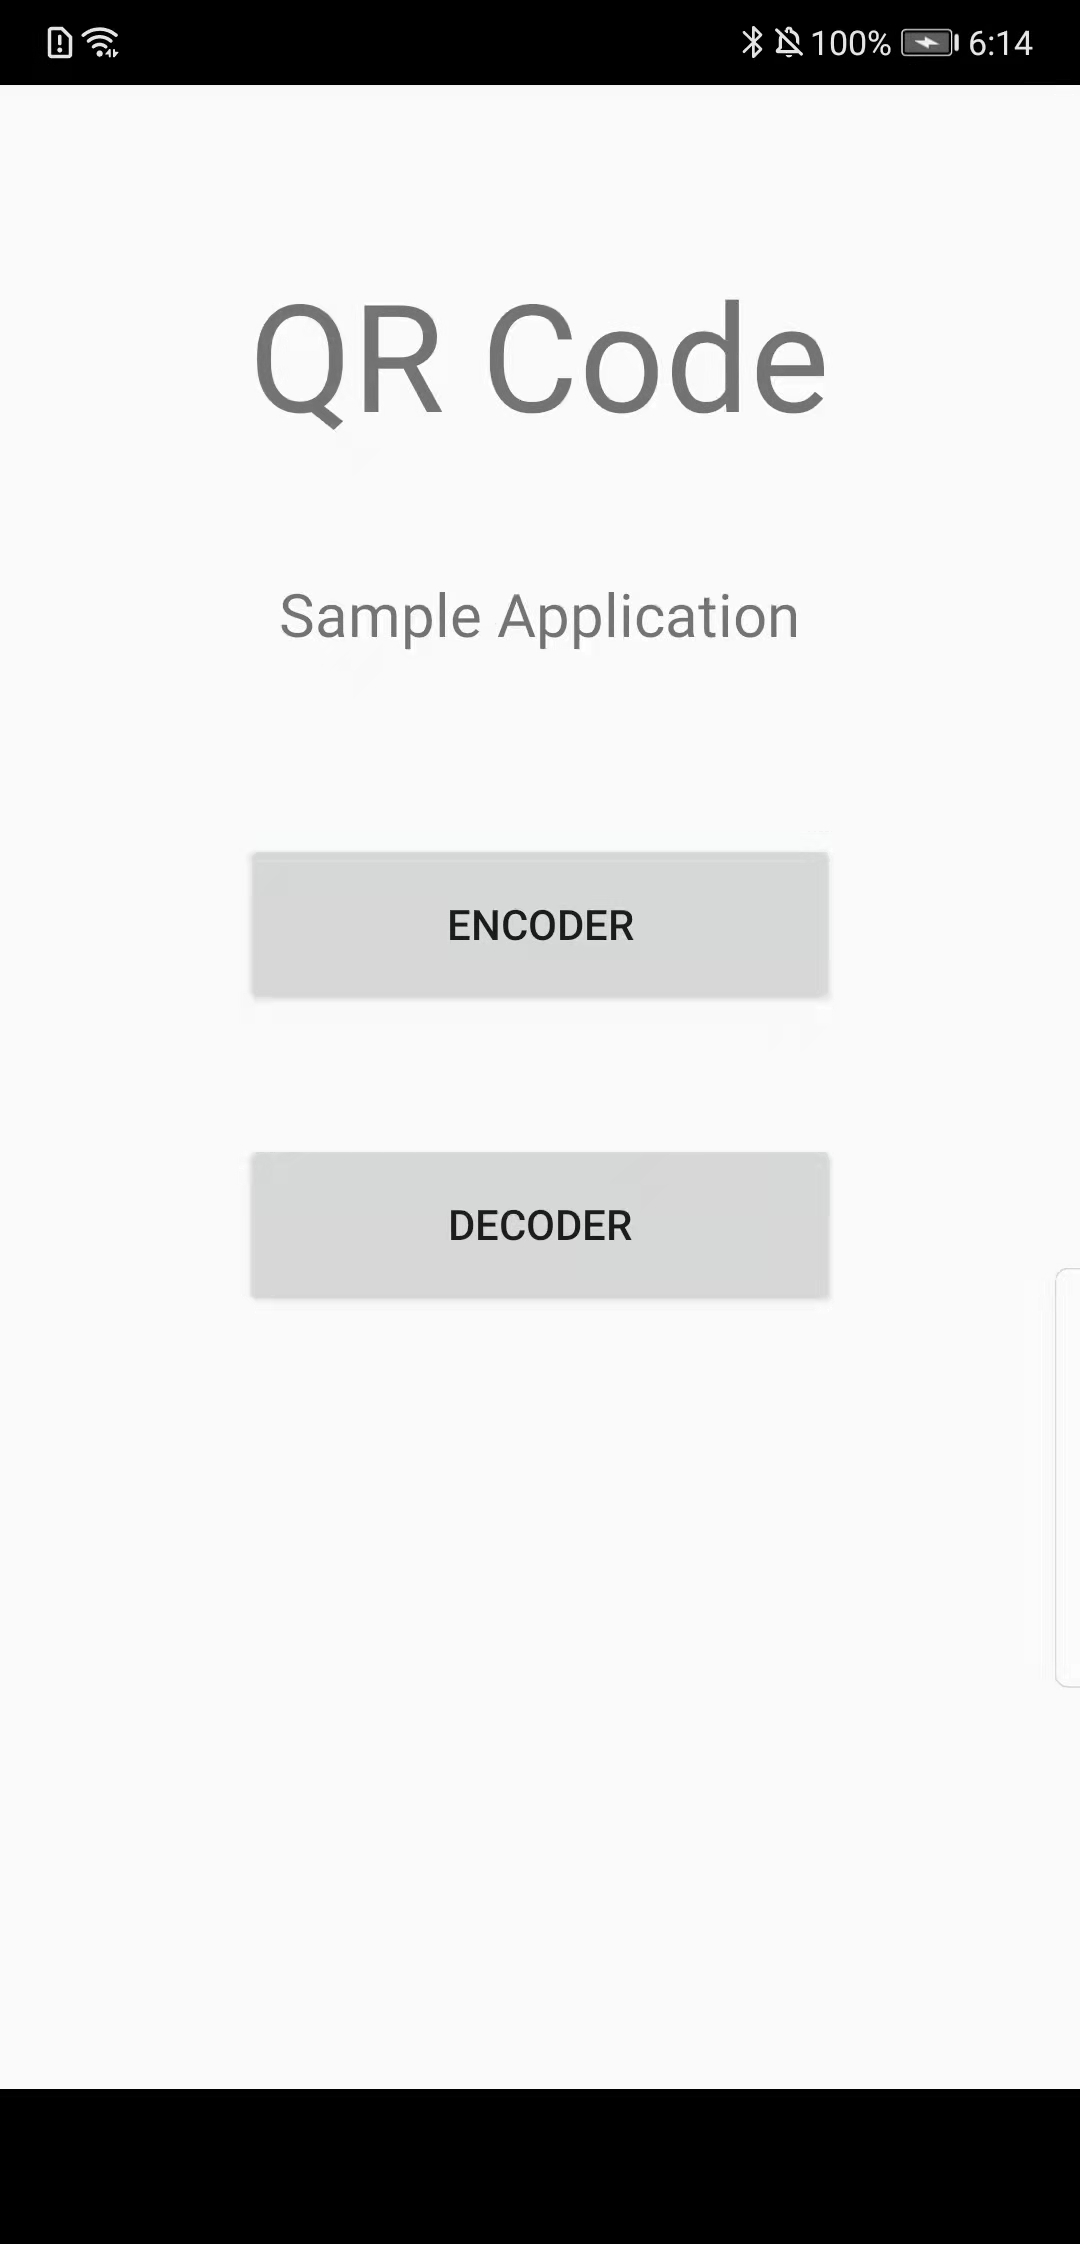
\includegraphics[width=\linewidth]{5-1.jpeg}
		\end{minipage}%
		\begin{minipage}[t]{0.25\linewidth}
		\centering
		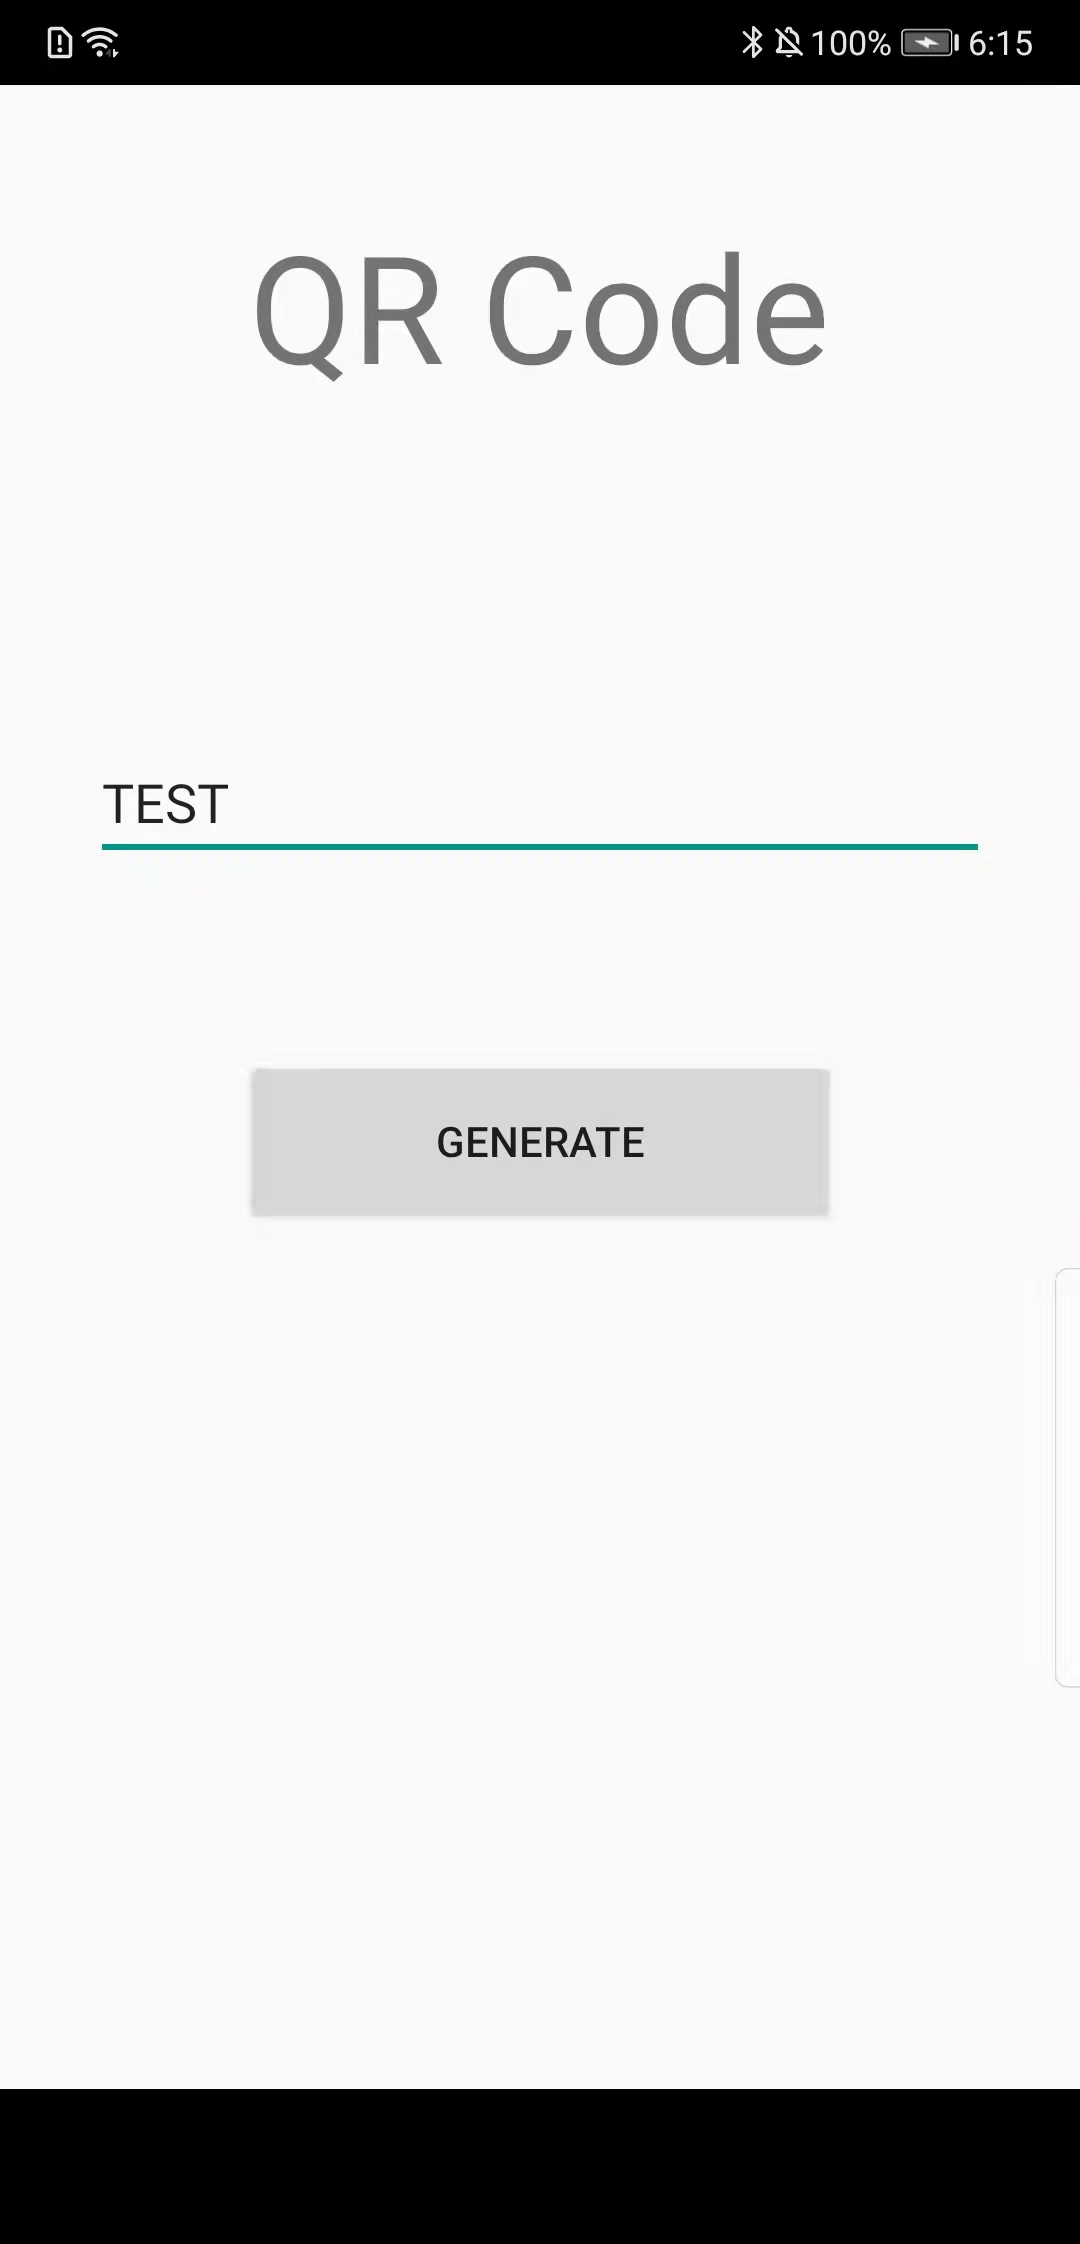
\includegraphics[width=\linewidth]{5-2.jpeg}
		\end{minipage}
	\linebreak
		\begin{minipage}[t]{0.25\linewidth}
		\centering
		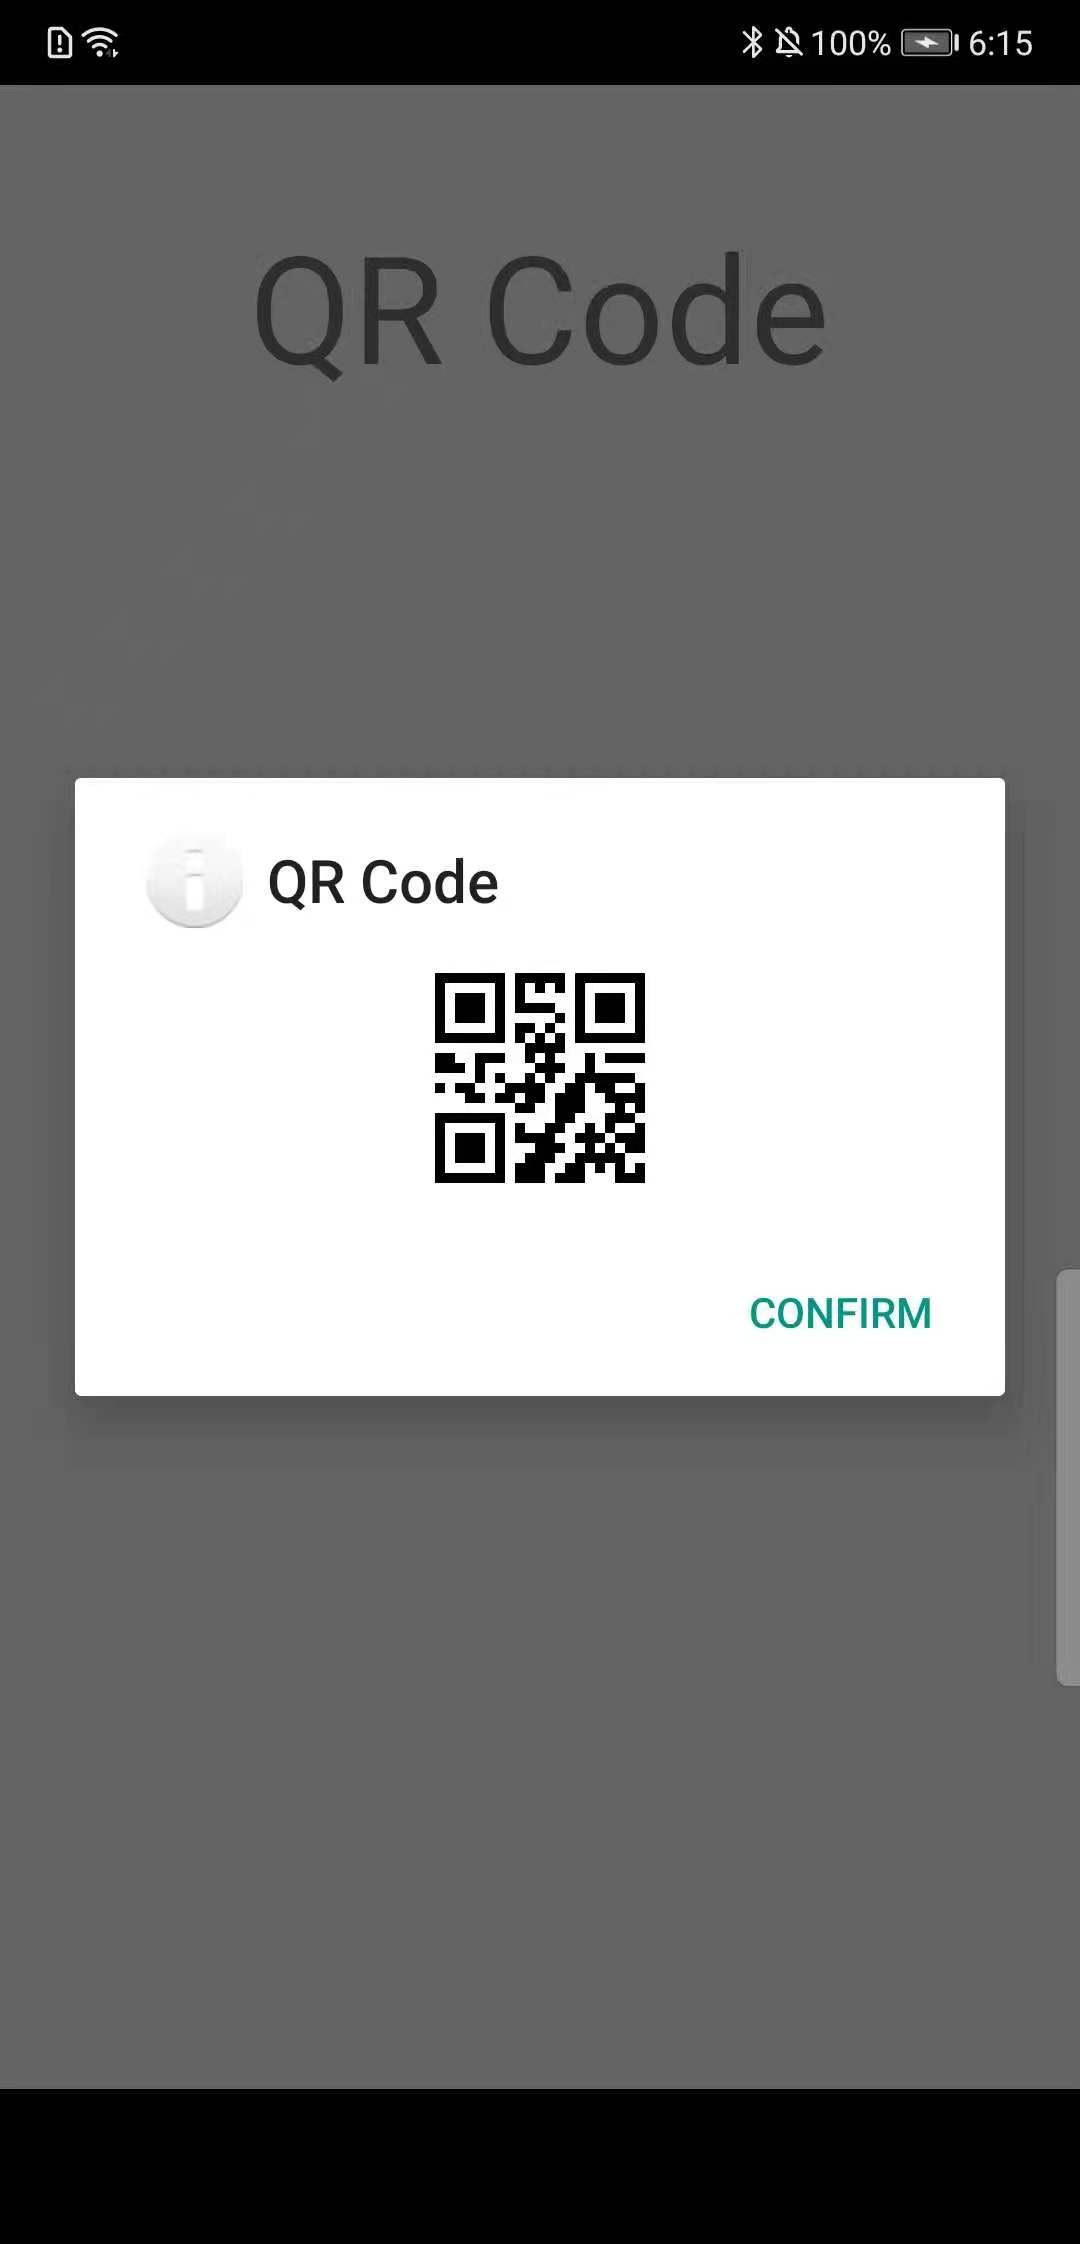
\includegraphics[width=\linewidth]{5-3.jpeg}
		\end{minipage}
		\begin{minipage}[t]{0.25\linewidth}
		\centering
		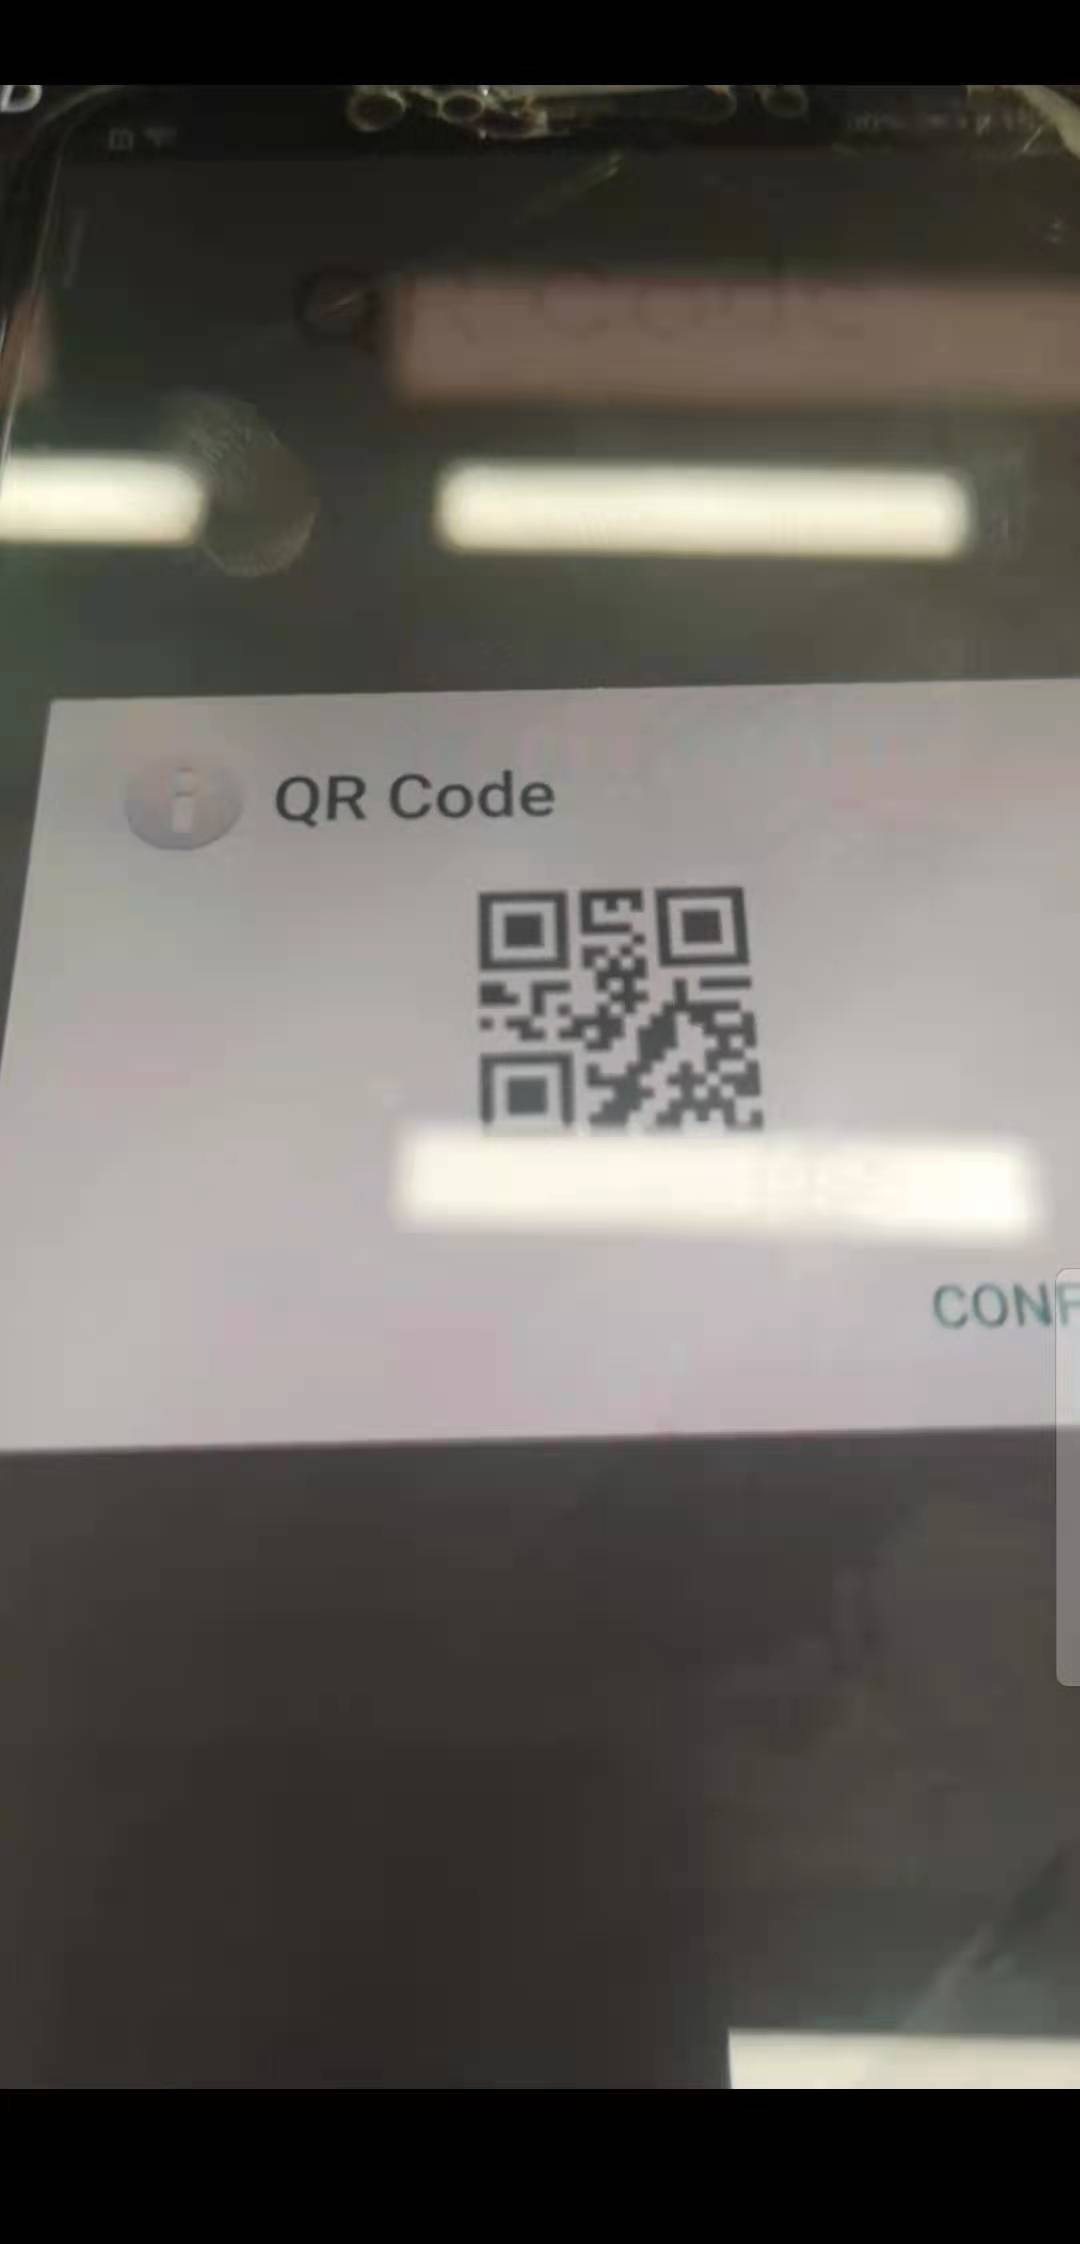
\includegraphics[width=\linewidth]{5-4.jpeg}
		\end{minipage}
		\begin{minipage}[t]{0.25\linewidth}
		\centering
		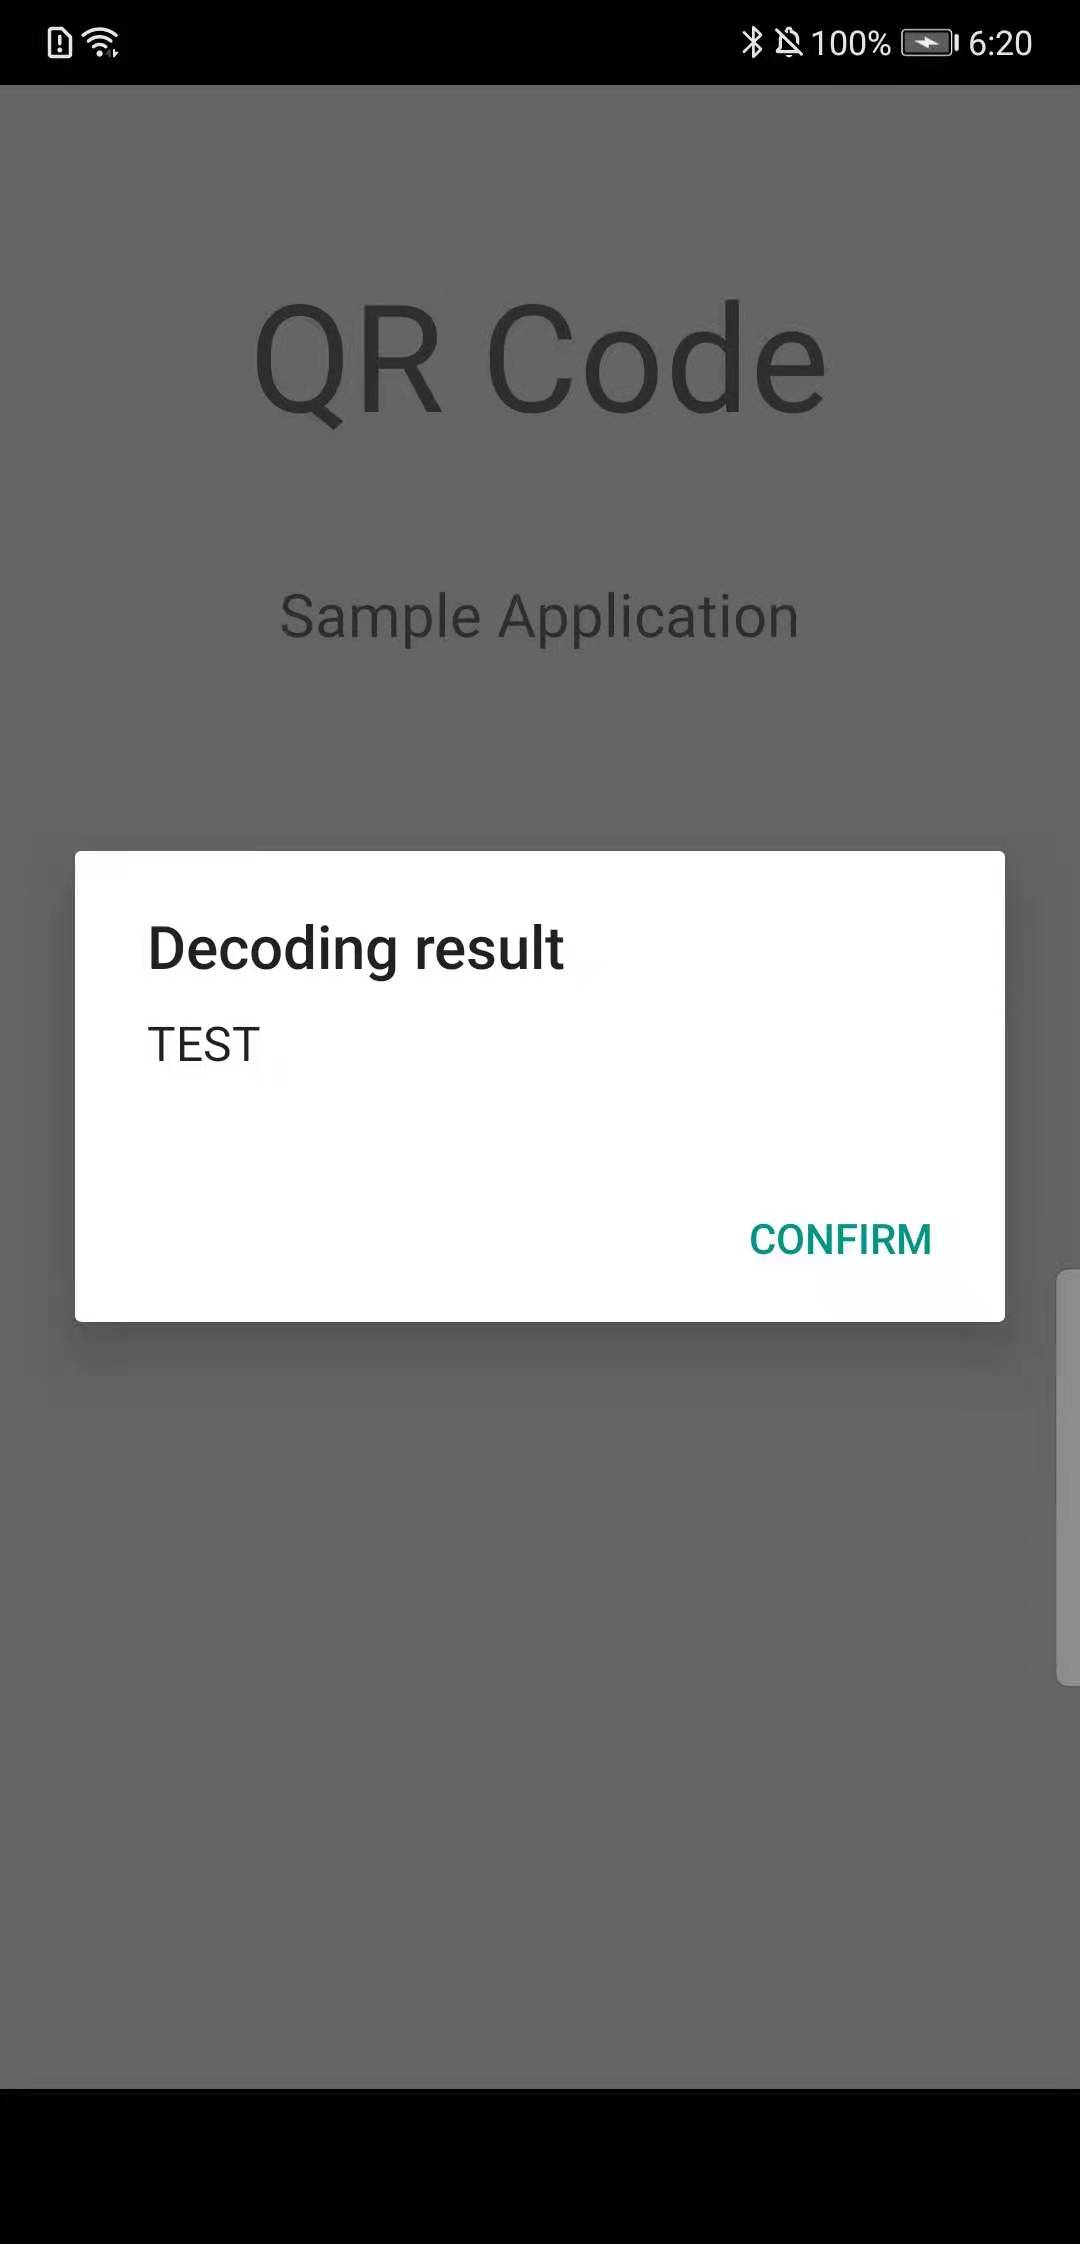
\includegraphics[width=\linewidth]{5-5.jpeg}
		\end{minipage}
	\caption{The main function of the initial application}\label{fig5}
\end{figure}

From a user's view, the application is not so convenient because:
\begin{itemize}
	\item It does not support saving the generated QR code into the mobile storage.
	\item It does not support detecting QR code from the pictures stored in the mobile.
\end{itemize}

Therefore, we propose our improved QR code application in the following sections.

\section{Code Explanation}
To improve the application, we first need to understand the logic of the initial application.

\subsection{MainActivity}
Notice that the function \texttt{onActivityResult()} in \texttt{MainActivity} appears for the first time, which aims to get the response from some other triggers or message passing. In the application, the function receive responces from \texttt{TestDecoder}. When  \texttt{TestDecoder} meets a valid QR code, it send the decoding result back and \texttt{MainActivity} make a \texttt{AlterDialog} to show the result.

Therefore, for \texttt{TestEncoder}, we just need to start the activity, and we call \texttt{StartActivity}; for \texttt{TestDecoder}, we need to start the activity and receive the responses, and according to the previous introduction, we should call \texttt{StartActivityForResult}.

\subsection{TestEncoder}
In \texttt{TestEncoder}, we just need to call the APIs provided by the zxing\footnote{\href{https://github.com/zxing/zxing}{https://github.com/zxing/zxing}} library. Basically, what we need to do is:
\begin{enumerate}
\item Get the text from the \texttt{EditText} module;
\item Call \texttt{MultiFormatWriter()} API provided by zxing library with the parameter of the text reading fro m the previous step.
\item Convert the returning \texttt{bitMatrix} into RGB colors and draw the pixels on a bitmap.
\item Put the bitmap on an \texttt{ImageView} object, and display the object on an \texttt{AlterDialog} to show the result.
\end{enumerate}

\subsection{TestDecoder}
In \texttt{TestDecoder}, we need to read the image stream from the camera and call the APIs provided by the zxing library to decode the QR code. The first function is implemented using \texttt{SurfaceView}, and the second function is implemented using the \texttt{QRCodeReader} object in the zxing lib.

For \texttt{SurfaceView}, the project implements three methods: \texttt{surfaceCreated}, \texttt{surfaceChanged} and \texttt{surfaceDestroyed}. The first one and the last one is similar to the constructor and destructor of an object, and the second method is called only when the format or size of the preview interface is changed, which allows us to dynamically detect the QR code in the camera image stream.

\section{Improvements}
\subsection{Save QR Code to Mobile Storage}

To enable saving QR code to mobile storage, we first modify the \texttt{AlertDialog} in \texttt{TestEncoder} to add a \texttt{save} button. When the user press the \texttt{save} button, the application will call our \texttt{save\_pics} method, which is implemented as follows.
\begin{lstlisting}[language=java]
private void save_pics(Bitmap bitmap) {
    String path = getApplicationContext().getFilesDir().getPath() 
                  + File.separator + "QRcode";
    File appDir = new File(path);
    if(!appDir.exists()) appDir.mkdirs();
    String filename = "QRCode" + System.currentTimeMillis() + ".jpg";
    File file = new File(appDir, filename);
    try {
        FileOutputStream fo = new FileOutputStream(file);
        bitmap.compress(Bitmap.CompressFormat.JPEG, 60, fo);
        fo.flush();
        fo.close();
        MediaStore.Images.Media.insertImage(
            getBaseContext().getContentResolver(), 
            file.getAbsolutePath(), filename, null);
        Uri uri = Uri.fromFile(file);
        getBaseContext().sendBroadcast(
            new Intent(Intent.ACTION_MEDIA_SCANNER_SCAN_FILE, uri));
    } catch (IOException e) {
            e.printStackTrace();
    }
}
\end{lstlisting}

Notice that saving the picture to the mobile storage takes three steps\footnote{\href{https://www.cnblogs.com/monkey0928/p/10716923.html}{https://www.cnblogs.com/monkey0928/p/10716923.html}}:
\begin{enumerate}
\item Save the picture first. In this step, we should add the permissions in the \texttt{AndroidManifest.xml} file of the project since we are accessing external storage. Therefore, we can add the following lines in the \texttt{AndroidManifest.xml} file:
\begin{lstlisting}
<uses-permission 
  android:name="android.permission.WRITE_EXTERNAL_STORAGE" 
/>
<uses-permission
  android:name="android.permission.READ_EXTERNAL_STORAGE" 
/>
\end{lstlisting}
\item Insert the picture to the system picture gallery. This step is vital since we need to let the Android system to find the pictures we have saved in the system. To achieve this goal, we just need to call the \texttt{MediaStore.Images.Media.insertImage} method.
\item Notify the picture gallery to update. We sent a broadcast to notify the system picture gallery to update using \texttt{Uri} and \texttt{sendBroadcast} method.
\end{enumerate}

Therefore, we have finished adding ``save QR code'' button in the encoding process.

\subsection{Detect QR Code from Pictures in the Gallery}
To enable detecting QR code from pictures in the gallery, we first add a button and make minor modifications to the layout of the \texttt{TestDecoder} interface. Then, we use \texttt{Intent.ACTION\_PICK} and \texttt{intent.setType("image/*")} method to get access to all the images in the mobile storage. Therefore, we just need to fetch the user-selected image and send it back to the main process. Here we reference some implementations of the \texttt{surfaceCreated} and use the \texttt{onActivityResult()} function we have introduced before. For detail of the implementation, refer to the source codes.

\section{Final Performance}
We use the same HUAWEI P20 mobile for real-world testing, and the main function of the our modified application is shown in Fig. \ref{fig6}.

\begin{figure}[htbp]
	\centering
		\begin{minipage}[t]{0.2\linewidth}
		\centering
		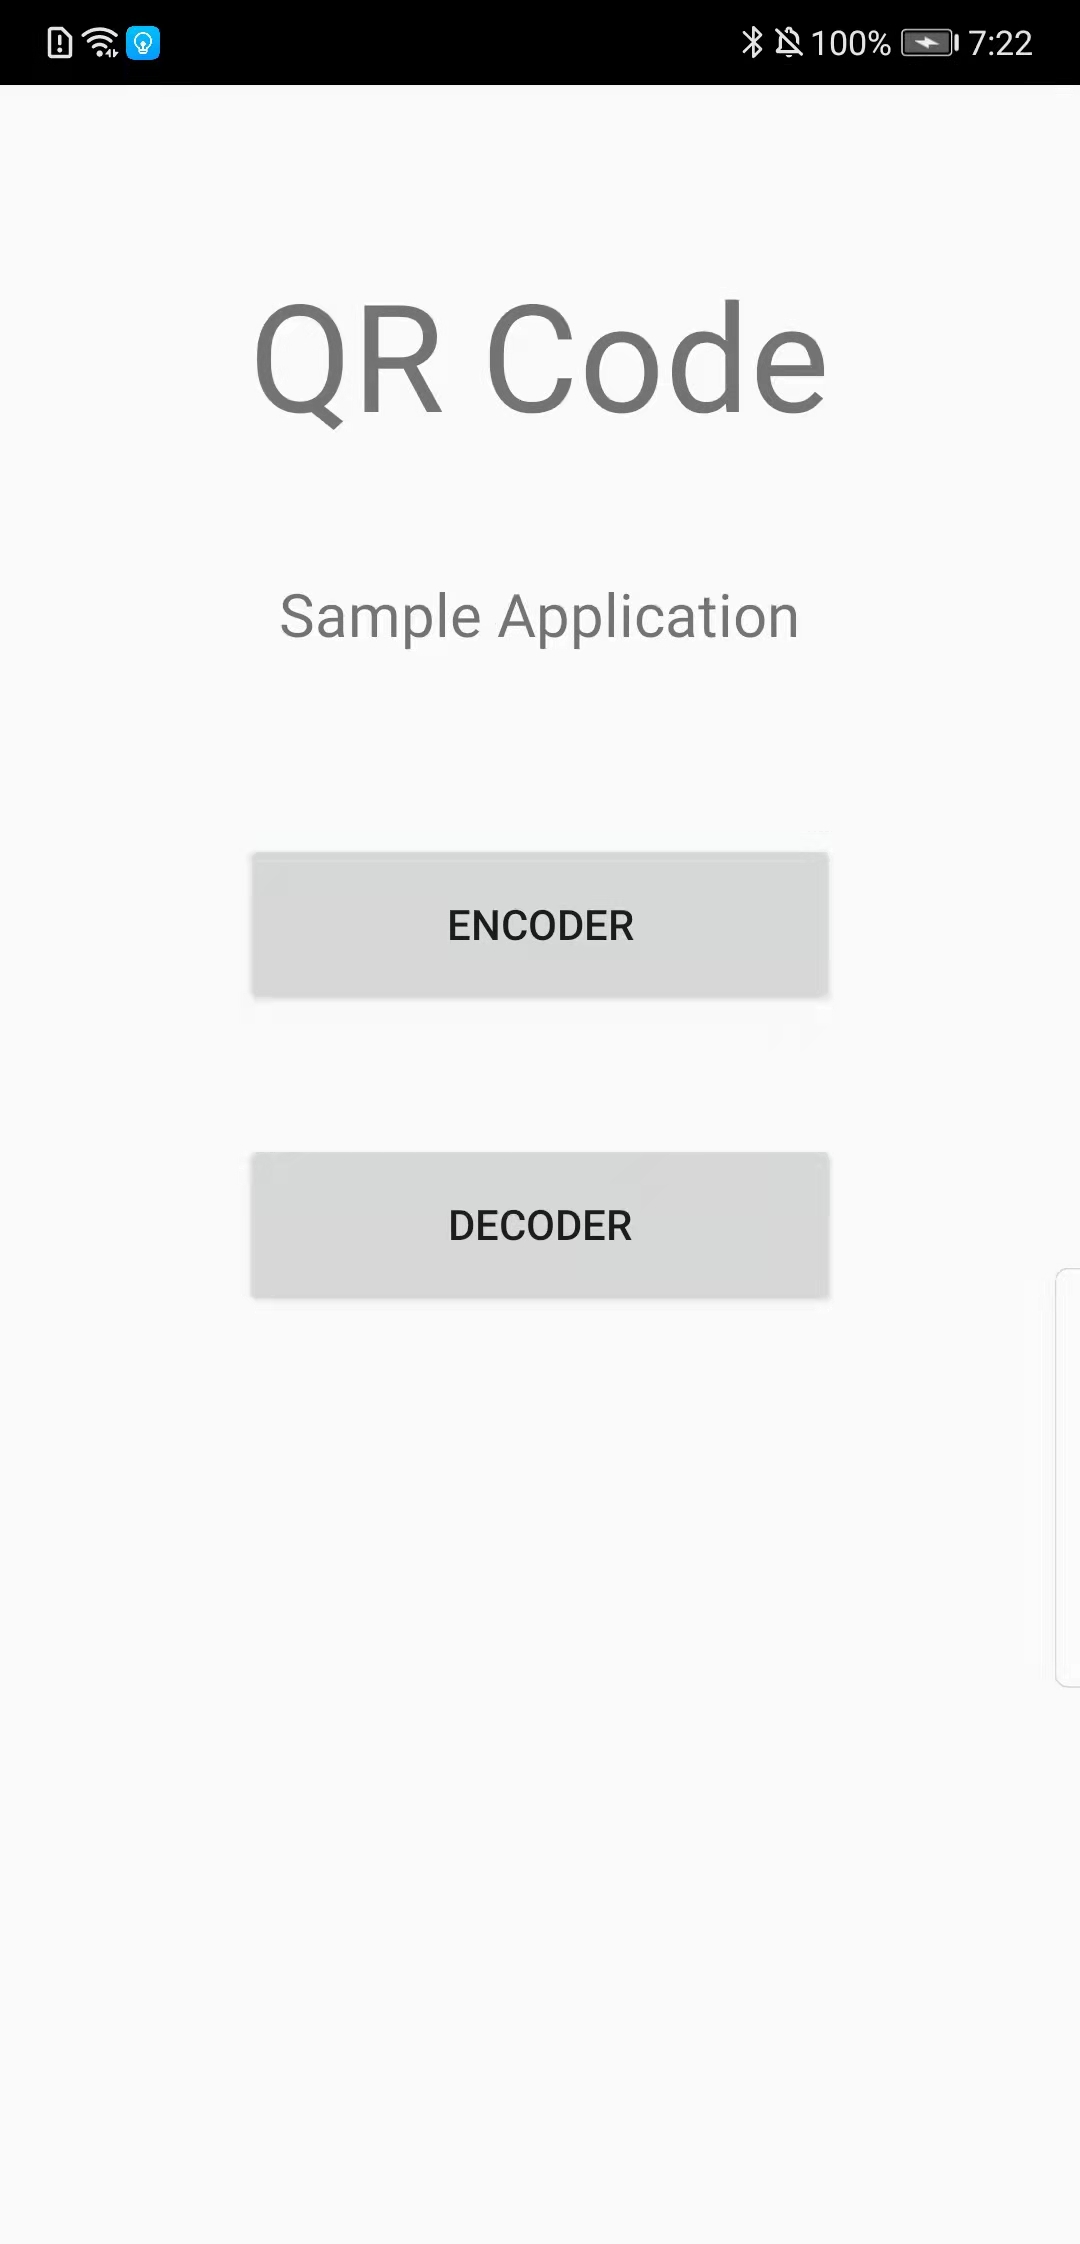
\includegraphics[width=\linewidth]{6-1.jpeg}
		\end{minipage}%
		\begin{minipage}[t]{0.2\linewidth}
		\centering
		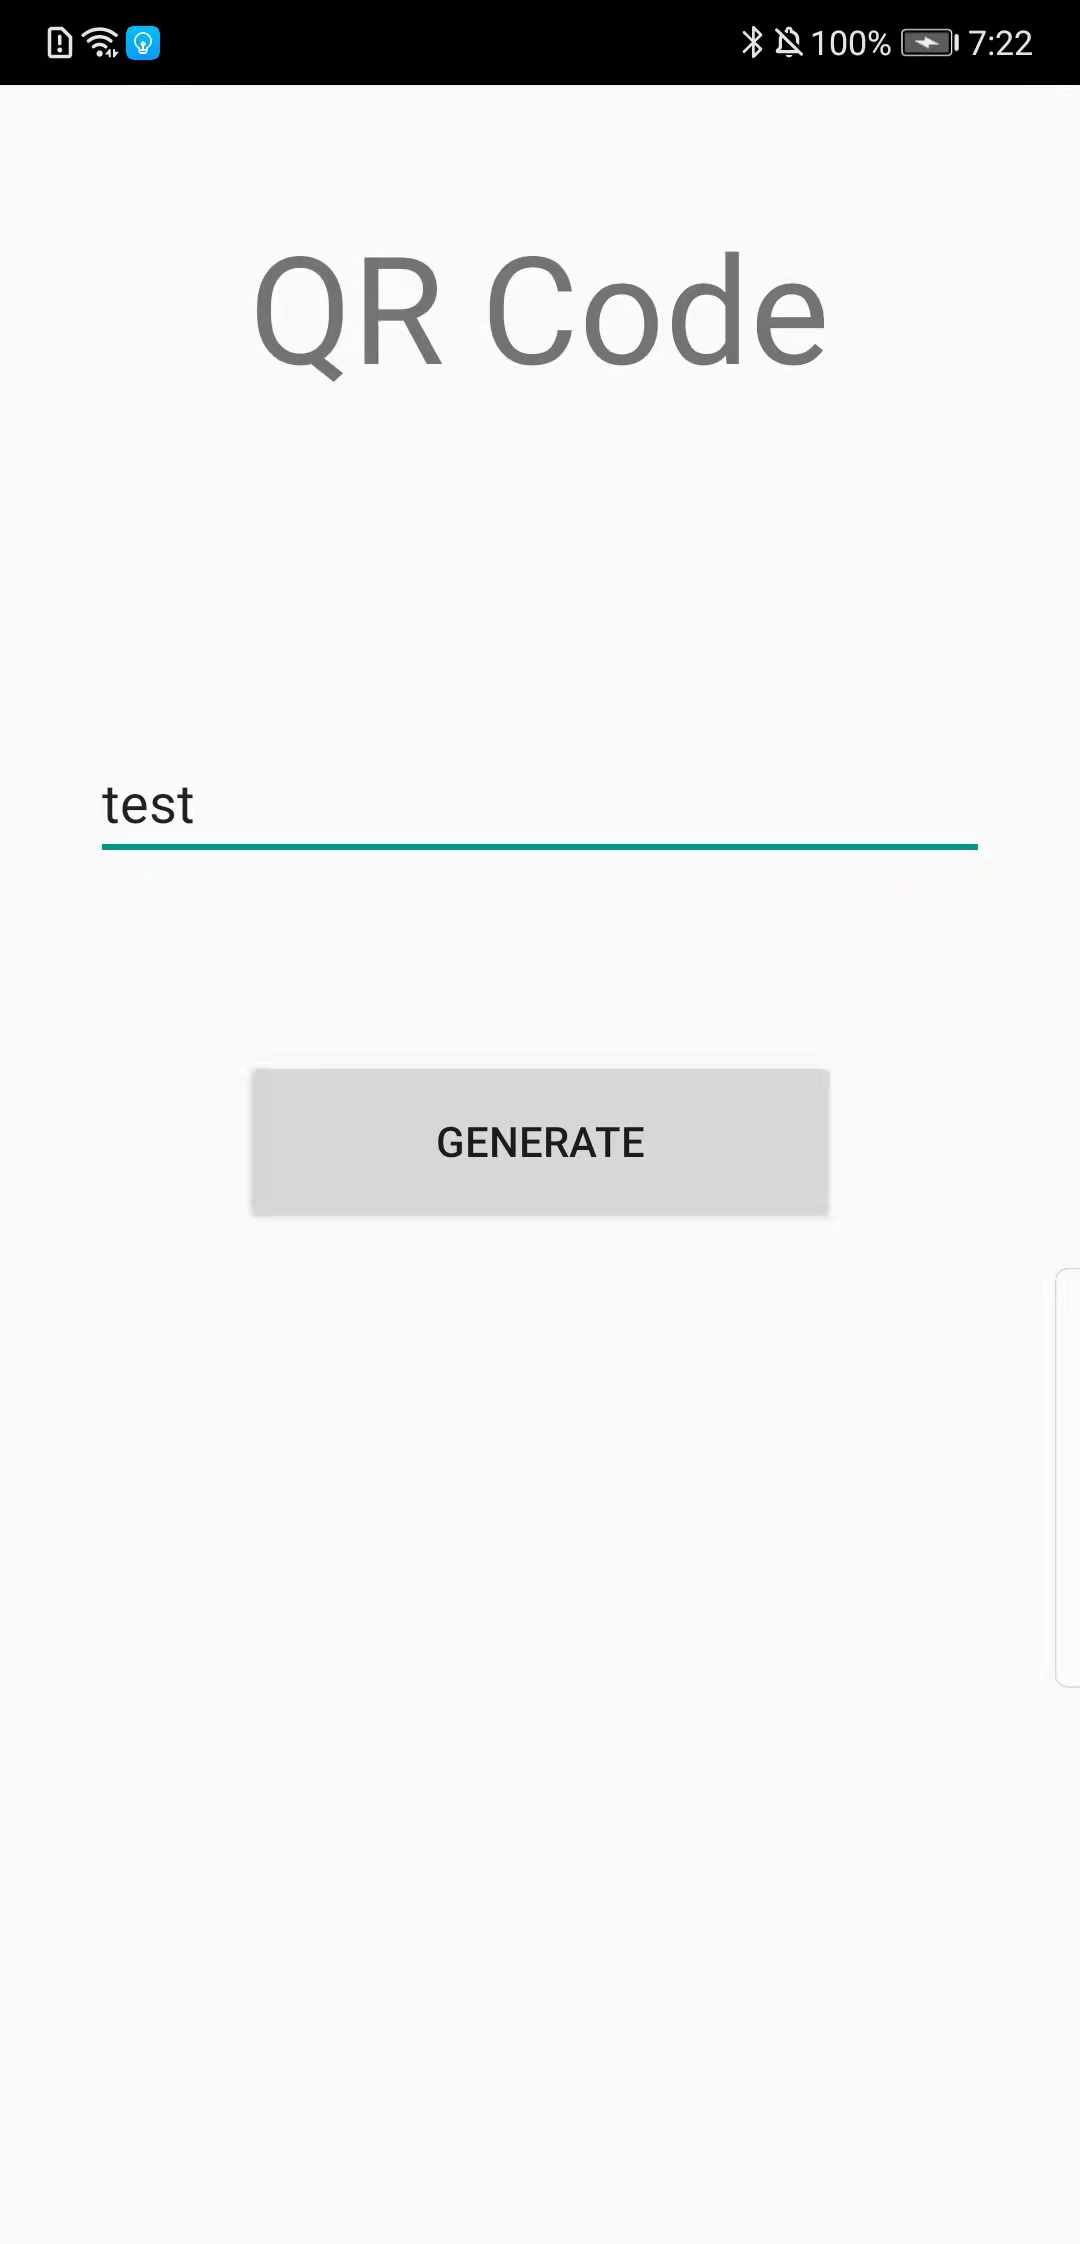
\includegraphics[width=\linewidth]{6-2.jpeg}
		\end{minipage}
		\begin{minipage}[t]{0.2\linewidth}
		\centering
		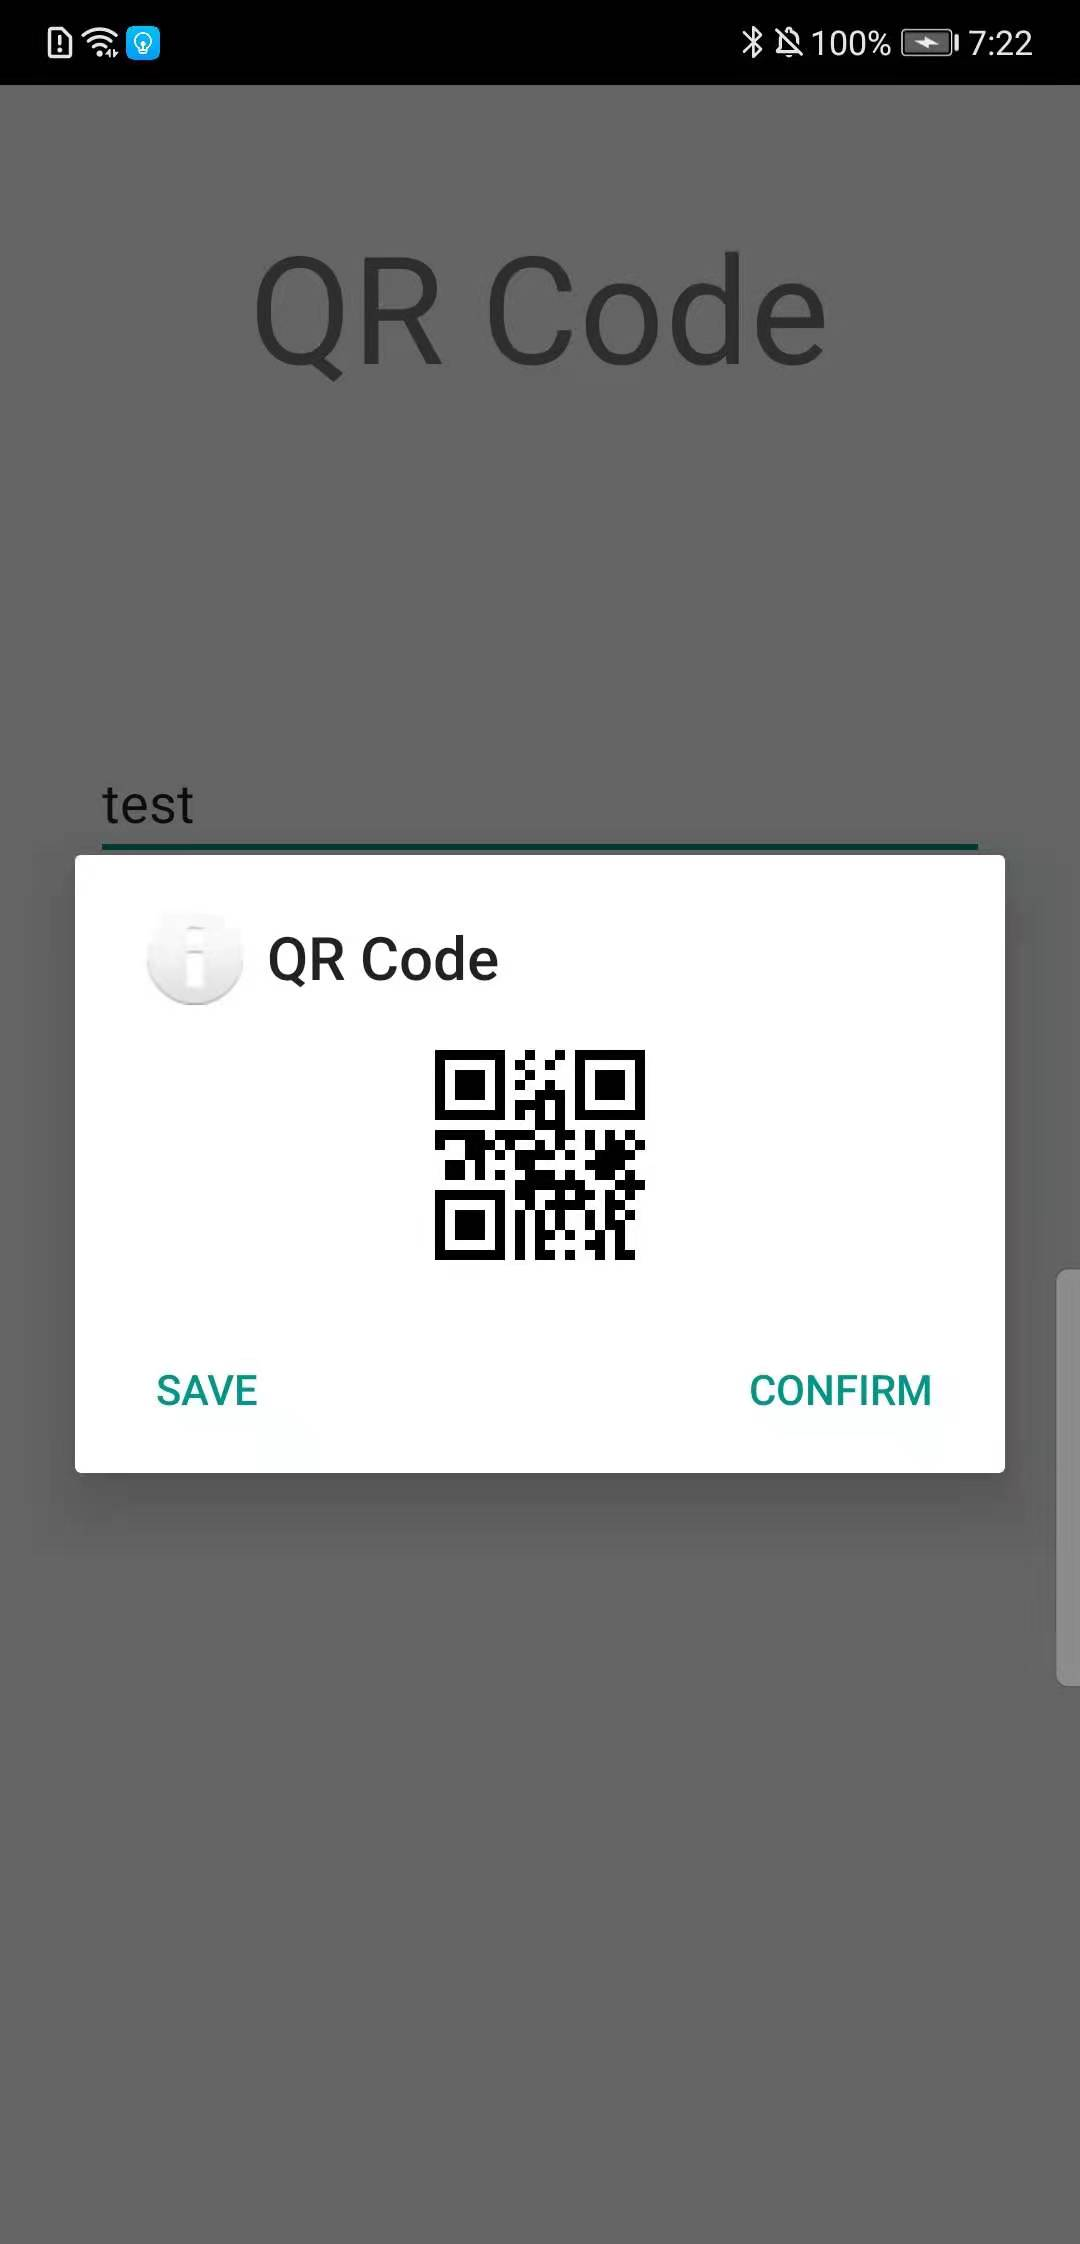
\includegraphics[width=\linewidth]{6-3.jpeg}
		\end{minipage}
	\linebreak
		\begin{minipage}[t]{0.2\linewidth}
		\centering
		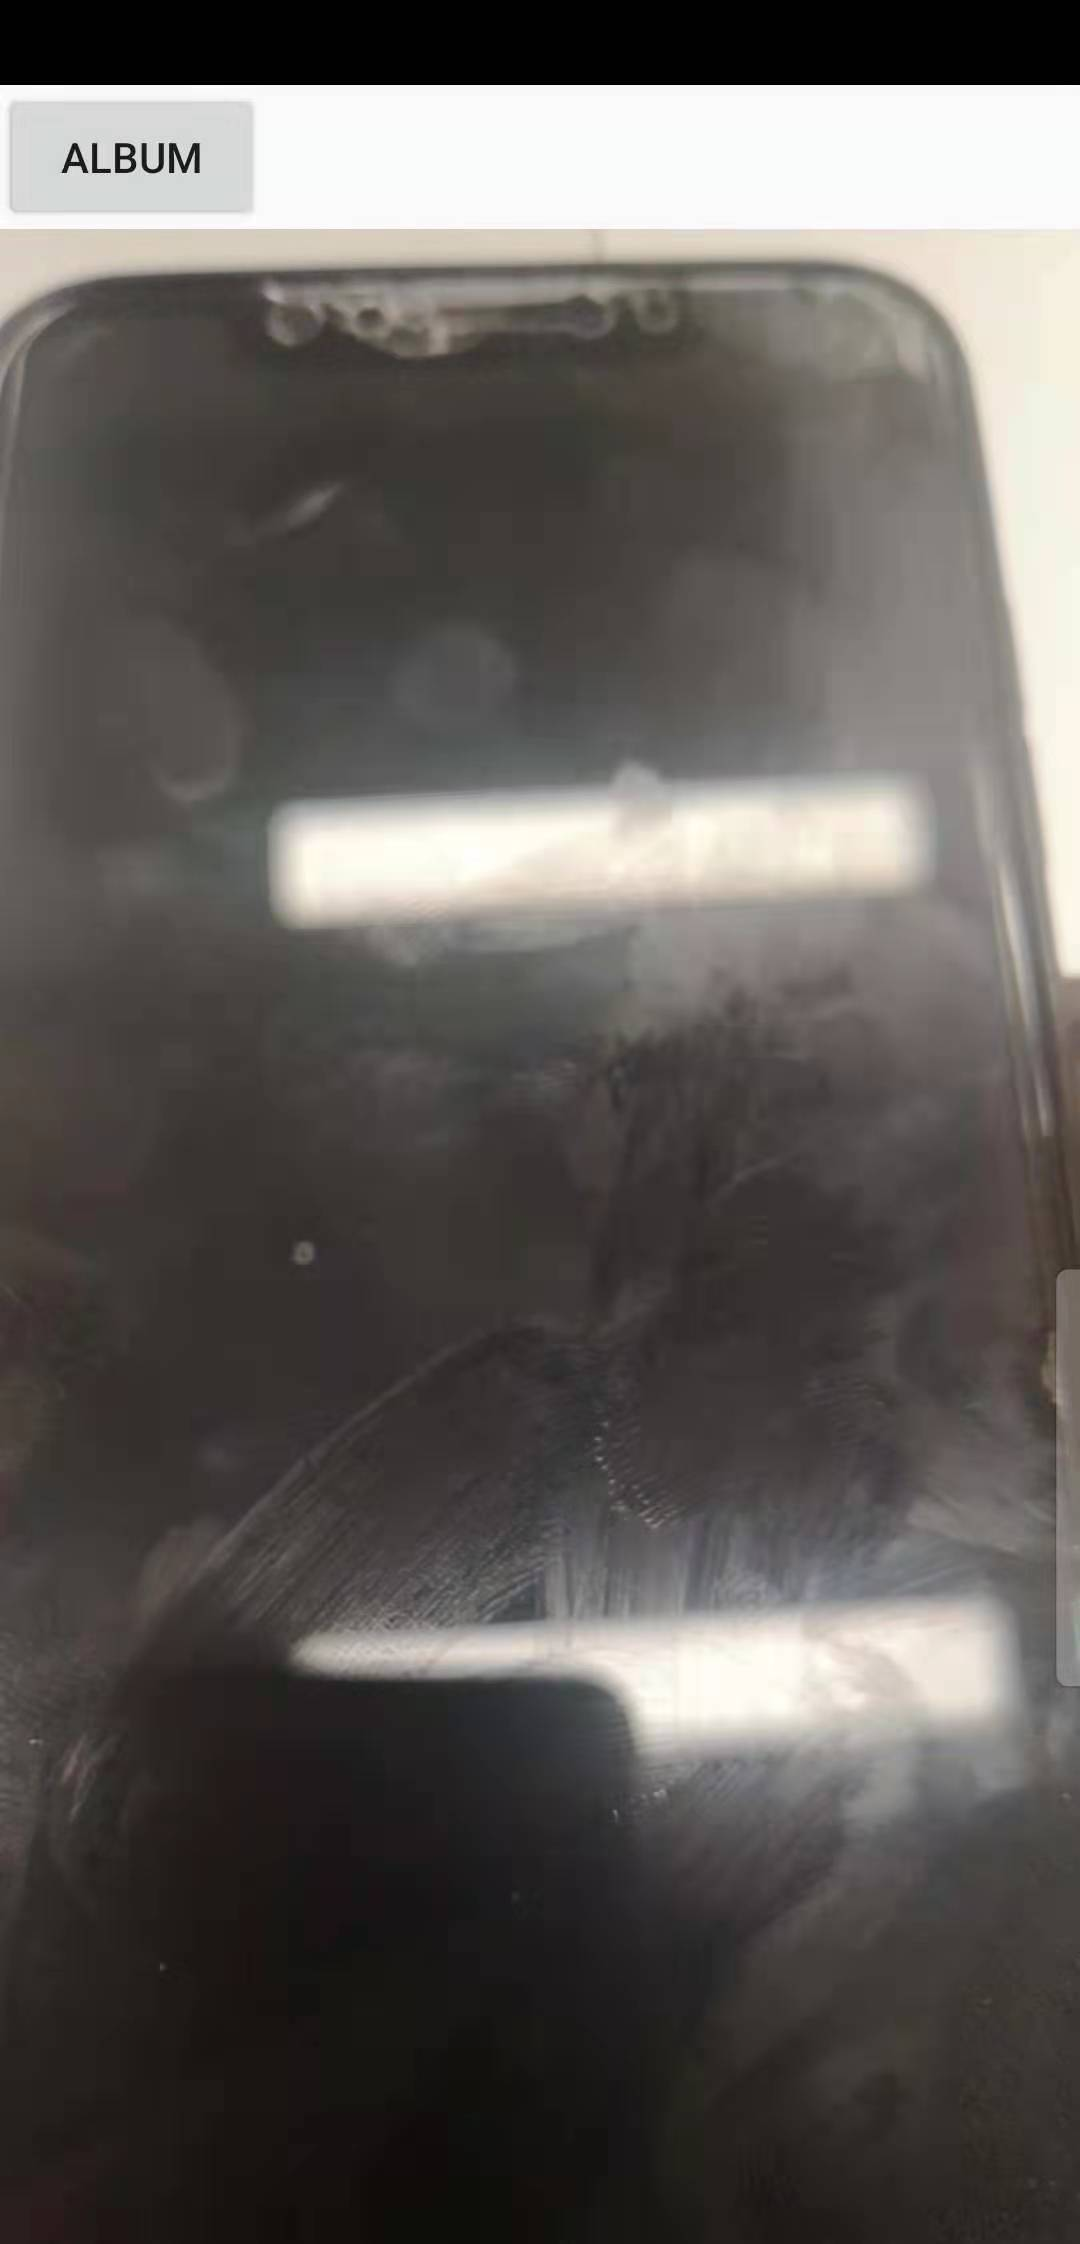
\includegraphics[width=\linewidth]{6-4.jpeg}
		\end{minipage}
		\begin{minipage}[t]{0.2\linewidth}
		\centering
		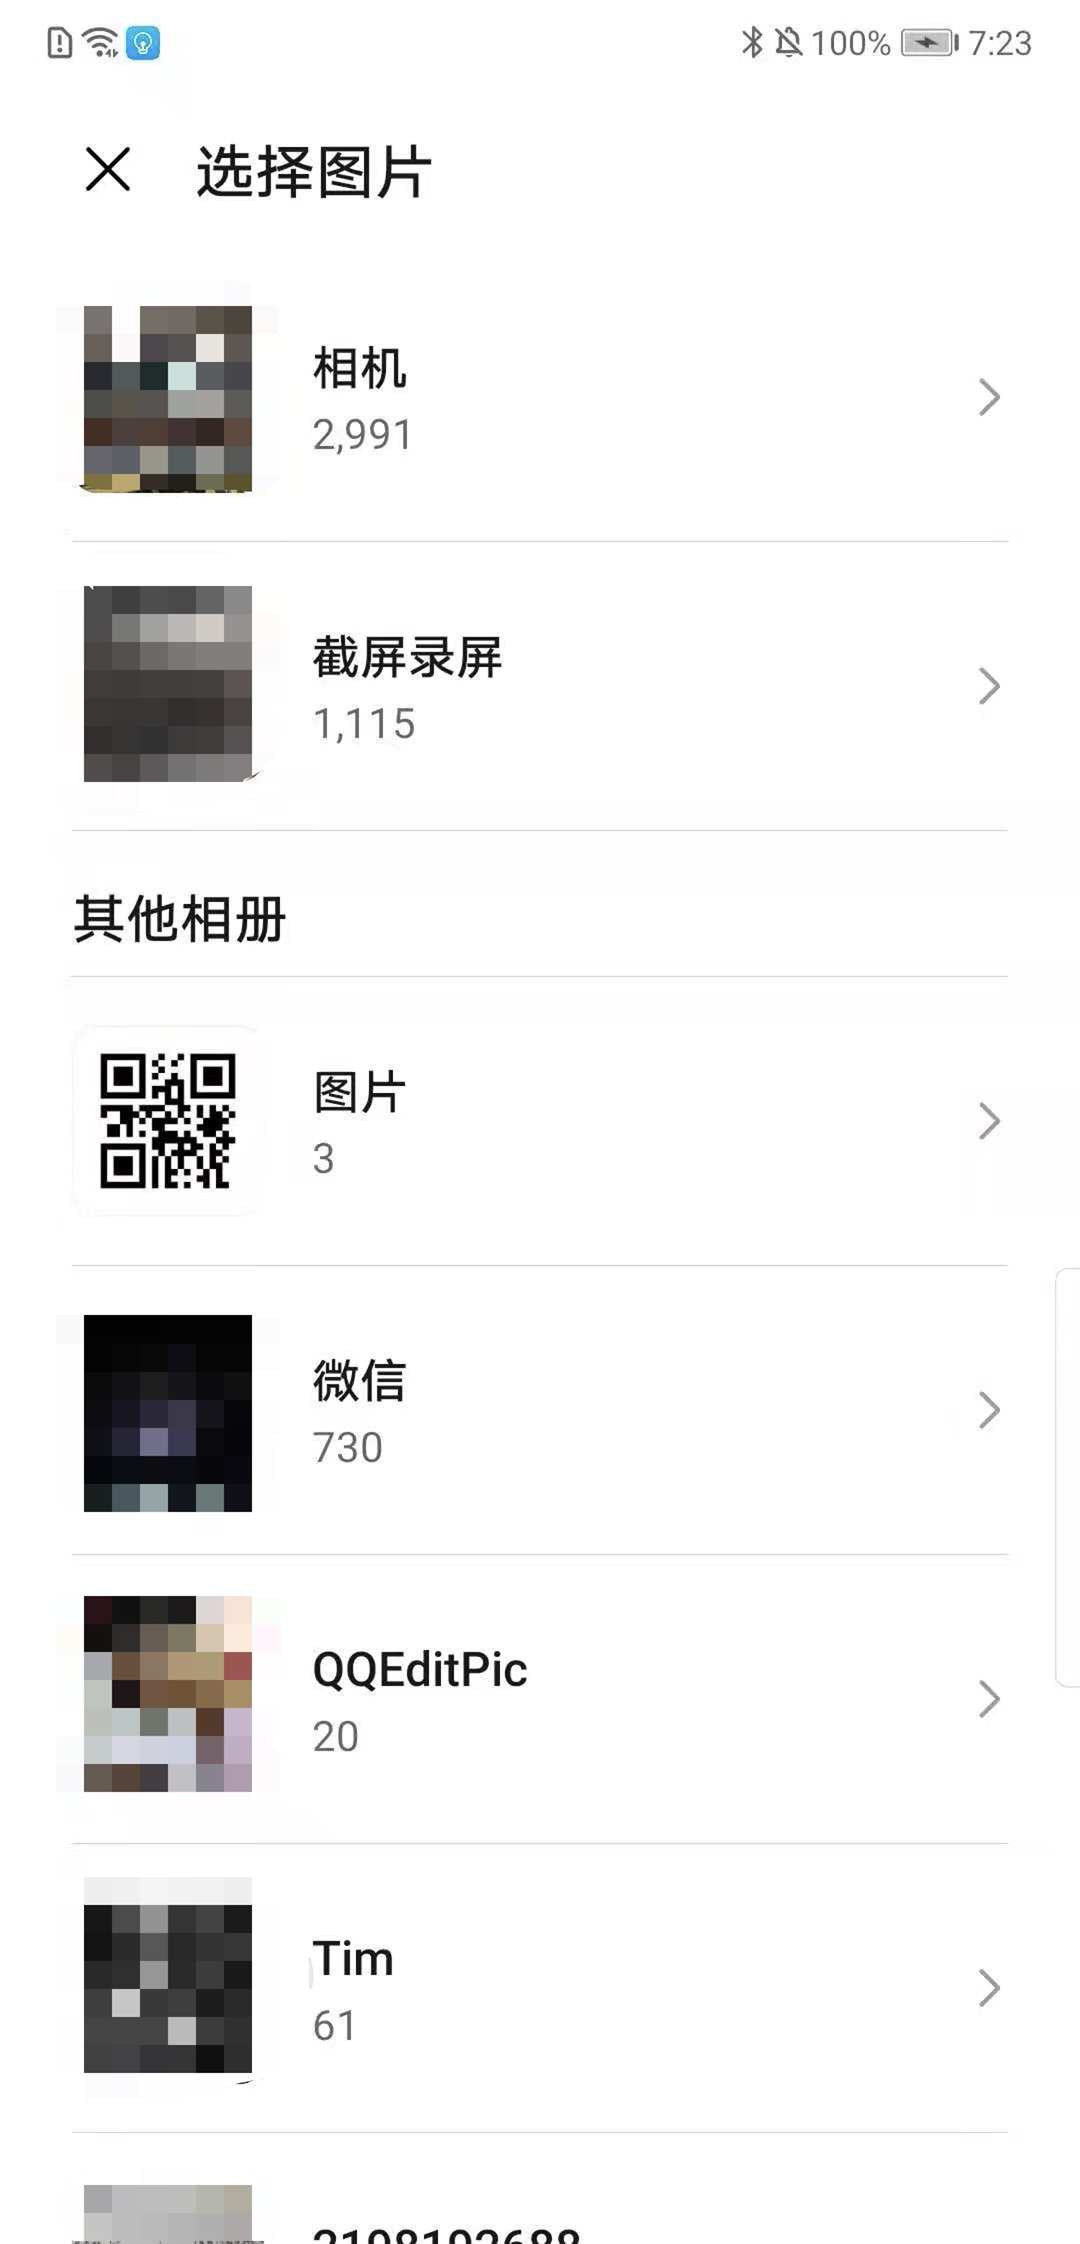
\includegraphics[width=\linewidth]{6-5.jpeg}
		\end{minipage}
		\begin{minipage}[t]{0.2\linewidth}
		\centering
		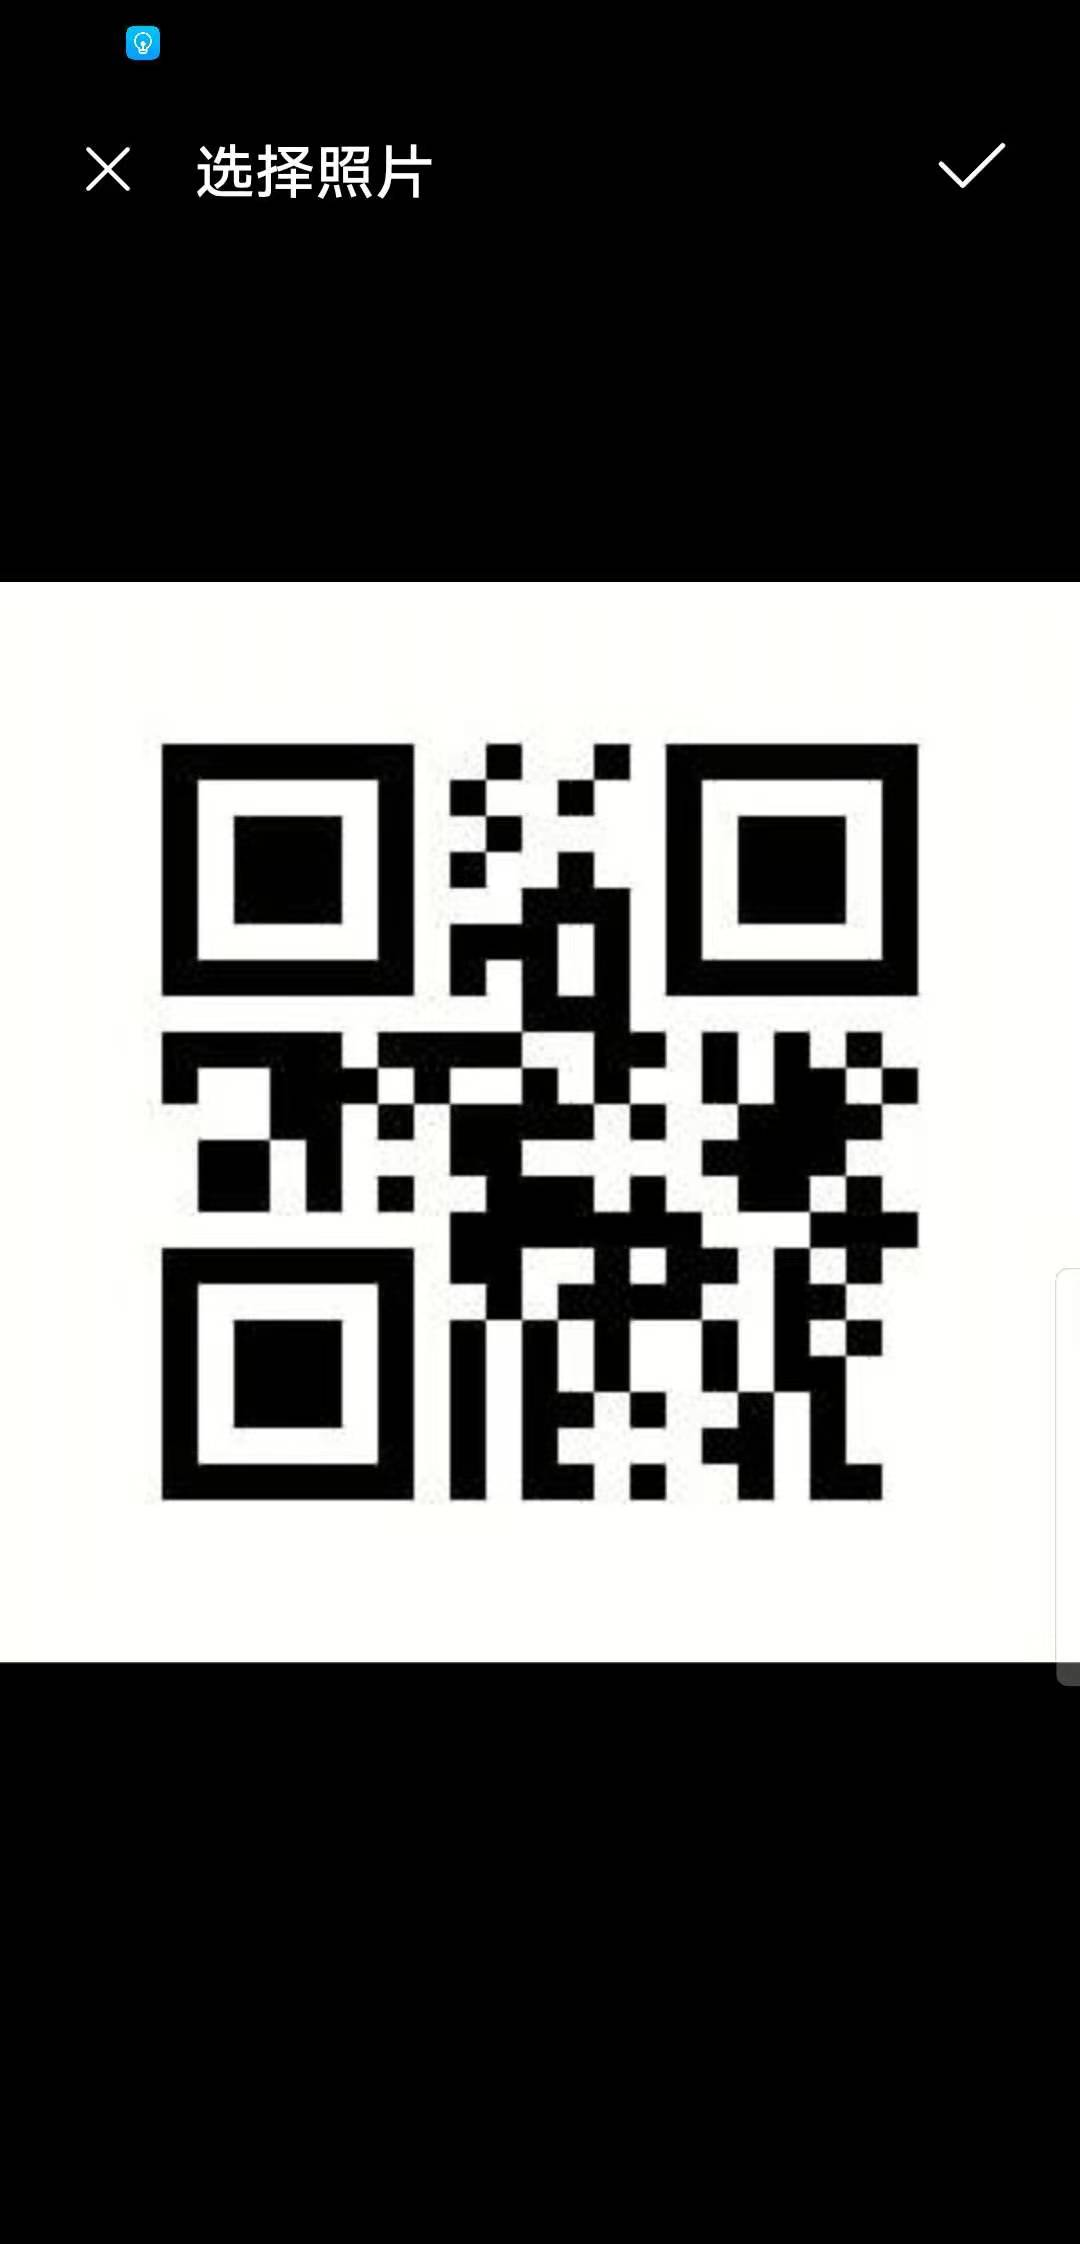
\includegraphics[width=\linewidth]{6-6.jpeg}
		\end{minipage}
		\begin{minipage}[t]{0.2\linewidth}
		\centering
		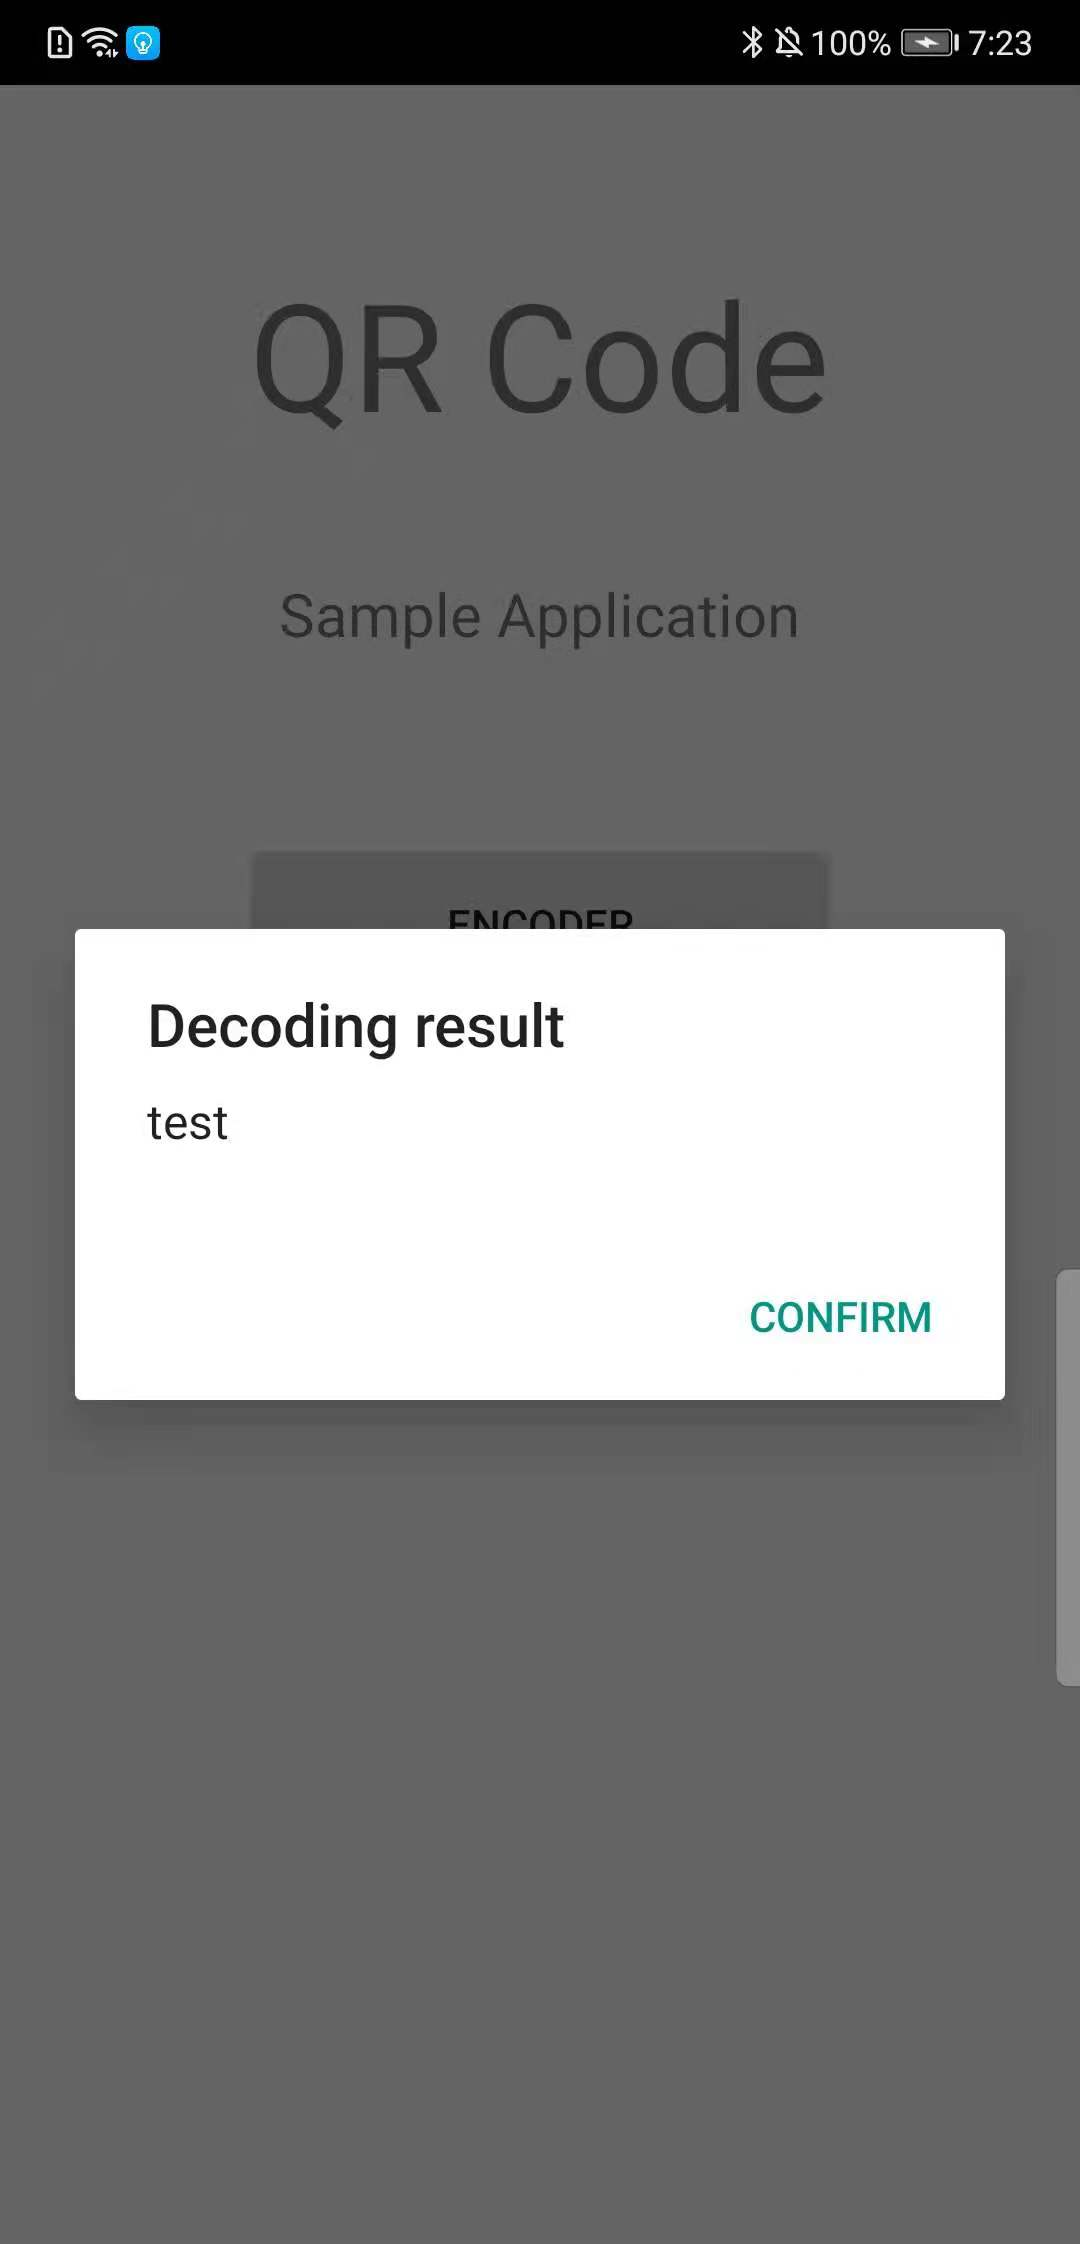
\includegraphics[width=\linewidth]{6-7.jpeg}
		\end{minipage}
	\caption{The main function of our modified application}\label{fig6}
\end{figure}

Our modified application has all the functions of the initial application. What's more, the two additional functions (saving the QR code to the mobile storage, and detecting QR code from pictures in the gallery) make the application handier, and more user-friendly. 

\section{Conclusion}
To complete this lab, I have read some materials about how to use zxing library. Moreover, I'm more familiar with the Android Studio to develop Android applications. After finishing the basic requirements of compiling and executing the application, I make some important modifications to make the application more user-friendly, such as saving QR code to the mobile storage and detecting QR code from the mobile gallery. Future work may include developing a prettier UI, supporting different types of QR code and redirect to the corresponding applications, such as Alipay and Wechat. I am looking forward to implement them in the future.

The full implementation codes of the lab is available in my \href{https://github.com/Galaxies99/EE447-CourseData/tree/main/Labs/Lab2}{github repository}.

%========================================================================
\end{document}
